%+----------------------------------------------------------------------------+
%| SLIDES: Longer presentation on my paper 1805.01696
%| Author: Antonio miti
%| Event: Visit in Salerno, March 2019
%+----------------------------------------------------------------------------+


%- HandOut Flag -----------------------------------------------------------------------------------------
\newif\ifHandout
	\Handouttrue  %uncomment for the printable version
	%Handling of flags it is not preserved when passing to standalone-subfiles!

%- D0cum3nt ----------------------------------------------------------------------------------------------
\ifHandout
	\documentclass[handout,10pt]{beamer}   
	\setbeameroption{show notes} %print notes    
\else
	\documentclass[10pt]{beamer}
\fi


%- Packages ----------------------------------------------------------------------------------------------
\usepackage{verbatim}
\usepackage{appendixnumberbeamer}
\usepackage[mode=buildnew,subpreambles=true]{standalone}
\usepackage{amsmath, amssymb}
\usepackage{tikz}
\usetikzlibrary{arrows,shapes,calc}
\usetikzlibrary{shapes.callouts}
\usepackage{tikz-cd}
\usepackage{graphicx, animate}
\usepackage{hyperref}
\usepackage[english]{babel}
\usepackage{csquotes}
\usepackage{stackengine}
\usepackage{fourier} %Danger Sign


%--Beamer Style-----------------------------------------------------------------------------------------------
\usetheme{toninus}

%- T1tle P4g3 -------------------------------------------------------------------------------------------
\title{Multisymplectic aspects of link invariants} 
\subtitle{(Based on \href{http://arxiv.org/abs/1805.01696}{Arxiv:1805.01696})}
\author[AMM]{\href{https://dmf.unicatt.it/miti/}{Antonio Michele Miti}\\(Joint work with Mauro Spera)}
\institute[UCSC and KU Leuven]{
  \begin{tabular}[h]{ccc}
      Università Cattolica del Sacro Cuore & & KU Leuven \\
      Brescia, Italy & & Leuven, Belgium \\
      \href{https://dipartimenti.unicatt.it/dmf-home?rdeLocaleAttr=it}{\includegraphics[width=3.5cm]{Logos/UnicattBS-logo}} & & 
      \href{https://wis.kuleuven.be/english}{\includegraphics[width=4cm]{Logos/KULeuven_logo}}
  \end{tabular}      
}
\date[Unisa_19] % (optional, should be abbreviation of conference name)
{	%(partly joint with: M.Spera)\\ 
	Fisciano, March 19, 2019
}




%Intermediate checkpoint slide
\newcommand{\checkpoint}[0]{
	%\ifHandout
	
	%\else
 	\begin{frame}{Outline}
  		%\tableofcontents[currentsection,currentsubsection]
  		\addtocounter{framenumber}{-1}
  		\tableofcontents[currentsection]
	\end{frame}
	%\fi
}
%--WORKAROUND------------------------------------------------------------------------------------------
%Credit: https://tex.stackexchange.com/questions/147899/path-problem-with-included-file-inside-of-a-standalone-file
\providecommand{\includestandalonewithpath}[3][]{%
  \begingroup%
  \providecommand{\datapath}{#2}%
  \includestandalone[#1]{\datapath/#3}%
  \endgroup}

%---------------------------------------------------------------------------------------------------------------------------------------------------
%- D0cum3nt ----------------------------------------------------------------------------------------------------------------------------------
\begin{document}
%-------------------------------------------------------------------------------------------------------------------------------------------------


%-------------------------------------------------------------------------------------------------------------------------------------------------
	\begin{frame}  % Alternative: \maketitle outside of frame
	  \titlepage
	  \ifHandout
		  \tikz[overlay,remember picture]
			{
	    		%	\node at ($(current page.west)+(1.5,0)$) [rotate=90] {\Huge\textcolor{gray}{\today}};
	    			\node[        draw,
	        			shape border rotate=90,
					isosceles triangle,
			        isosceles triangle apex angle=90,
	        			fill=yellow]
	        		at ($(current page.north east)-(1,1)$) [rotate=-45] {\textcolor{red}{Annoted version}};
			}
	\fi
	\end{frame}
	\addtocounter{framenumber}{-1}
\note{
	\scriptsize{
	\textbf{\underline{Abstract}}\\
		The present talk is a survey of part of recent joint work with Mauro Spera\cite{Miti2018} (arXiv: 1805.01696), in which we investigated some connections between multisymplectic geometry and knot theory.
		\vspace{0.05em}
		
		A connection between these two topics can be established via mechanics of ideal fluids.\\
		The key idea is to regard the group of orientation-preserving diffeomorphism of the Euclidean space (corresponding to spatial configurations of an ideal incompressible fluid permeating the whole space) as a multisymplectic action on $\mathbb{R}^3$ with the standard volume form seen as a 2-plectic form.
		\vspace{0.5em}
		
		As a first result, we can explicitly construct a homotopy co-momentum map (à la Callies,  Fregier, Rogers and Zambon \cite{Callies2016}) associated to this multisymplectic action showing that it correctly transgresses to the standard hydrodynamical co-momentum map defined by Arnol’d, Marsden and Weinstein and others.
		\vspace{0.5em}
		
		The transition to knots occurs when one considers vortex filaments in hydrodynamics.\\
		It is possible to associate to these peculiar configurations of the fluid suitable conserved quantities, as defined by Ryvkin, Wurzbacher and Zambon\cite{Ryvkin2016}.\\
		These quantities are directly related to the Gauss linking number of the link supporting the vorticity.
		\vspace{0.5em}
		
		Time permitting, we shall discuss a reinterpretation of the (Massey) higher order linking numbers in terms of conserved quantities within the \cite{Ryvkin2016} multisymplectic framework, giving rise to knot theoretic analogues  of first integrals in involution.
		}
}
%---------------------------------------------------------------------------------------------------------------------------------------------------

%--------------------------------------------------------------------------------------------------------------------------------
\begin{frame}{Scope}
%\smartdiagram[circular diagram]{	Multisymplectic geometry,	Hydrodynamics,	Knot theory}
	\underline{Idea:}Multisymplectic Methods in Knot theory via Hydrodynamics.
	\vfill
\begin{center}
	\includestandalone{Pictures/Figure_PaperLogic}
\end{center}
\end{frame}
\note{
			\textbf{\underline{OUTLINE}}:
			\tableofcontents
}
%---------------------------------------------------------------------------------------------------------------------------------------------------


%--------------------------------------------------------------------------------------------------------------------------------
\section{Multisymplectic geometry and homotopy moment maps} 
\checkpoint
%+----------------------------------------------------------------------------+
%| SLIDES: Longer presentation on my paper 1805.01696
%| Chapter: Brief introduction to multisymplectic geometry and Homotopy momap
%| Author: Antonio miti
%| Event: Visit in Salerno, March 2019
%+----------------------------------------------------------------------------+

%- HandOut Flag -----------------------------------------------------------------------------------------
\newif\ifHandout
	\Handouttrue  %uncomment for the printable version

%- D0cum3nt ----------------------------------------------------------------------------------------------
\documentclass[beamer,10pt]{standalone}
	%\setbeameroption{show notes}
	




%- Packages ----------------------------------------------------------------------------------------------
%\usepackage{verbatim}
\usepackage[mode=buildnew,subpreambles=true]{standalone}
\usepackage{import}
\usepackage{amsmath, amssymb}
\usepackage{tikz}
%\usetikzlibrary{arrows,shapes,calc}
%\usetikzlibrary{shapes.callouts}
\usepackage{tikz-cd}
\usepackage{hyperref}
\usepackage[english]{babel}
\usepackage{stackengine}

%--Beamer Style-----------------------------------------------------------------------------------------------
\usetheme{toninus}



%--Beamer Style-----------------------------------------------------------------------------------------------
\usetheme{toninus}





%---------------------------------------------------------------------------------------------------------------------------------------------------
%- D0cum3nt ----------------------------------------------------------------------------------------------------------------------------------
\begin{document}
%------------------------------------------------------------------------------------------------


  \subsection{Multisymplectic manifolds}
  \begin{frame}[fragile]{Multisymplectic Manifold} %Fragile -->workaround tikzcd
			\begin{defblock}[$n$-plectic manifold]
			\includestandalone[width=0.95\textwidth]{Pictures/Figure_multisym}	
			\end{defblock}

			\begin{defblock}[(Weekly) Non-degenerate n-form]
				\begin{columns}
					\hfill
					\begin{column}{.4\linewidth}
						\centering{
						The multi-contraction map $\alpha^{(j)}$\par
						is injective in the case $j=1$.
						}
					\end{column}
					\begin{column}{.6\linewidth}
						\[
						\begin{tikzcd}[column sep= small,row sep=0ex]
						    \alpha^{(j)} \colon& \mathfrak{X}^j(M) 	\arrow[r]& 				\Omega^{n+1-j}(M) \\
						  						& \xi_1\wedge\ldots\wedge\xi_j 						\arrow[r, mapsto]& 	\iota_{\xi_j}\cdots\iota_{\xi_1} \omega 					
						\end{tikzcd}	
						\]
					\end{column}
				\end{columns}
			\end{defblock}

			\begin{itemize}
					\item multisymplectic means \emph{going higher} in the rank of $\omega$\pause
					\item 1-plectic $=$ symplectic
			\end{itemize}
			\vspace{1ex}
			\pause
			\begin{block}{Example:}
				Any oriented $(n+1)$-dimensional manifold is $n$-plectic w.r.t. the volume form.
			\end{block}			 


  \end{frame}
  \note[itemize]{
  	\item Notation: in the following, we will suppress $M$ when denoting the spaces of tangent fields $\mathfrak{X}(M)$ and differential forms $\Omega^n(M$)
  	\item Remark: introducing the notation of multi-contraction could seem an overkill at this point. However it will be useful in the following.
  	%Hiny by Ori
  	\item Weak is an $\infty$-dimensional condition on sections. Usually (for instance in the tautological form construction) is used a stronger condition:\\
		The bundle map $\alpha: TM \rightarrow \wedge^n M$, acting on fibers as
		$\alpha_x : v_x \to \iota_{v_x} \omega_x$
		is injective on every fibers.  
		\item the strong implies the weak: a bundle map between bundles on the same base induce a map between sections.
		\item The converse is not true. Consider $\omega = x \text{d}x \wedge \text{d}y$, a presymplectic form that is not degenerate only on a dense domain.
		The map induced on section is injective
		$$\Gamma(T\mathbb{R}^2) \rightarrow \Gamma(T^\ast\mathbb{R}^2) : f\partial_x + g\partial_y \to x \left(f \text{d}y - g \text{d} x\right)$$
		because the r.h.s. vanish only when $f,g$ are zero on $\mathbb{R}^2 \ \text{y-axis}$ but since $f,g$ are coefficient of smooth field, the continuity implies that such functions vanish everywhere.
		
		}
%---------------------------------------------------------------------------------------------------------------------------------------------------
	
%------------------------------------------------------------------------------------------------
\begin{frame}[fragile]{MS geometry and classical field mechanics}
		Consider a smooth manifold $Y$,
		\begin{columns}
			\hfill
			\begin{column}{.5\linewidth}
				\emph{Multicotangent bundle} $\bigwedge = \bigwedge^n T^\ast Y$\\
				is naturally $n$-plectic
			\end{column}
			\begin{column}{.4\linewidth}
				\[
				\begin{tikzcd}
					\Lambda \ar[d,"\pi"'] & T \Lambda \ar[d,"T \pi"] \ar[l] \\
					Y								& T Y \ar[l]
				\end{tikzcd}	
				\]
			\end{column}
		\end{columns}
	\pause
	\begin{defblock}[Tautological $n$-form]
		$\theta \in \Omega^n(\Lambda)$ such that:
		\begin{displaymath}
		\begin{split}
			\left[ \iota_{u_1 \wedge \ldots \wedge u_n} \theta \right]_\eta 
			&= \iota_{(T \pi)_\ast u_1 \wedge \ldots \wedge (T \pi)_\ast u_n} \eta \\
			&= \iota_{u_1 \wedge \ldots \wedge u_n} \pi^\ast \eta 
			\qquad \qquad \forall \eta \in \Lambda \, , \: \forall u_i \in T_\eta \Lambda 		
		\end{split}
		\end{displaymath}
	\end{defblock}
	\vfill
	\begin{columns}
		\begin{column}{.6\linewidth}
			\begin{defblock}[Tautological (multisymplectic) (n+1)-form]
				$$\omega := d \theta$$
			\end{defblock}
		\end{column}
		\begin{column}{.4\linewidth}
		 	\begin{claimblock}$\omega$ is not degenerate.\end{claimblock}	
		\end{column}
	\end{columns}	
	\pause
	\begin{keywordblock}
		\begin{tabular}{|c|c|c|}
			\hline 
			point-particles mechanics & $\rightsquigarrow$ & classical fields mechanics \\
			%(finite discrete DOF) & & (finite dimensional continuous DOF) \\
			\hline 
			symplectic & $\rightsquigarrow$ & multisymplectic \\ 
			\hline 
			Observables (Poisson) algebra & $\rightsquigarrow$ & Observables $L-\infty$ algebra
			 \\ 
			\hline 
			Co-moment map & $\rightsquigarrow$ & Homotopy co-momentum map \\ 
			\hline 
		\end{tabular} 
	\end{keywordblock}

	
\end{frame}
\note[itemize]{
	\item This example is significant from the perspective of geometric classical field theory:
		\begin{displaymath}
			\frac{\text{classical mechanics}}{\text{symplectic geo.}} =
			\frac{\text{classical field mechanics}}{\text{multisymplectic geo.}}
		\end{displaymath}
	\item Multicotangent bundle is the \emph{Higher analogue} of the cotangent bundle.
	(but it is not yet the analogue of a \emph{phase space}.)
\item The multiphase space is the sub-bundle of $n$-forms vanishing when contracted with 2 vertical fields.
  	\item The reason why this sub-bundle has a particular role is that it can be proved to be isomorphic to a suitable dual of the first Jet bundle.
  	\item For further details see Gotay et al. \href{https://arxiv.org/abs/physics/9801019}{arXiv:physics/9801019}. For a pictorial representation of all the structures involved in the geometric mechanics of I order classical field theories see appendix, pag: \ref{frame:Gimmsy}.
}
%------------------------------------------------------------------------------------------------	
	
%------------------------------------------------------------------------------------------------
\begin{frame}{Special classes of smooth objects} 
  	\begin{columns}
		\begin{column}[t]{.42\linewidth}		
			\begin{defblock}[Hamiltonian v.f.]
				$\mathfrak{X}_{ham} =  \left\lbrace X \in  \mathfrak{X} \right\vert \left. \iota_x \omega \textrm{ exact}  \right\rbrace$ 			
			\end{defblock}
			\begin{defblock}[Multisymplectic v.f.]
				$\mathfrak{X}_{ms} =  \left\lbrace X \in  \mathfrak{X} \right\vert \left. \mathcal{L}_X \omega = 0  \right\rbrace$ 	
			\end{defblock}
		\end{column}
		\begin{column}[t]{.58\linewidth}		
			\begin{defblock}[Hamiltonian $(n$-$1)-$forms]
				\begin{displaymath}
					\Omega^{n-1}_{ham} 	:=
					\biggr\{ H \in  \Omega^{n-1} \; \left\vert \; 
					\stackanchor{$\exists X \in \mathfrak{X}_{ham}$}{: $d H = -\iota_X \omega$} \right\} 
			\end{displaymath}
			\end{defblock}		
		\end{column}
  	\end{columns}
  	%
  	\vspace{0.5em}
  	%
  	\onslide<2->{
  	\begin{columns}
		\begin{column}[t]{.5\linewidth}	
			\centering\emph{Global symmetries}
			\begin{defblock}[Multisymplectic (Lie group) action]
				$\Phi: G \circlearrowright (M, \omega)$ \emph{right action} s.t. \\
				$$\hat{\Phi}(g)_\ast \omega = \omega \quad \forall g \in G$$
			\end{defblock}
		\end{column}
		\begin{column}[t]{.5\linewidth}			
			\centering\emph{Infinitesimal symmetries}
			\begin{defblock}[Multisymplectic (Lie algebra) action]
				$V: \mathfrak{g} \rightarrow \mathfrak{X} (M)$ \emph{Lie algebra morphism} s.t. \\
				$$\mathcal{L}_{V_\xi} \omega = 0 \quad \forall \xi \in \mathfrak{g}$$	
			\end{defblock}
		\end{column}
  	\end{columns}
  	}
  	%
  	\onslide<3->{		
	  	\begin{asideblock}[Hierarchy of conserved quantities]%Shades of...
	  		\begin{table}[] % http://tablesgenerator.com/
			\begin{tabular}{lllll}
					& strictly conserved & & & $\mathcal{L}_X \alpha= 0$ \\
				$\alpha \in \Omega^\bullet$ & globally conserved & along $X \in \mathfrak{X}$ & $\Leftrightarrow$ & $\mathcal{L}_X \alpha\in B $ (exact) \\
				  & locally conserved  & & & $\mathcal{L}_X \alpha\in Z $ (closed)                                
			\end{tabular}
			\end{table}
	  	\end{asideblock}
  	}
  	
  \end{frame}
  \note[itemize]{
  	\item Exactly as it happens in symplectic geometry, fixing a smooth form $\omega$ on $M$ yields a criterion for classifying vector fields and differential forms.
  	\\(Pay attention to the sign convention in defining the Hamiltonian vector fields)
  	\item Also, we can naturally select a special class of symmetries (global and infinitesimal) which preserve the fixed multisymplectic form.
  	\item Aside, we can start to see that, in this setting, measurable quantities are not only smooth functions but also differential forms with degree greater then zero.
  	For such objects can be defined weaker notions of conservation along a flow.
  	\item The idea to consider forms of various degree as observables do not fall out of the sky. 
  		For instance in a string there will be two kind of measurable quantities: extensive observable (1-forms), like the density, and intensive observables (0-forms), like the tension. 
 		%\href{https://en.wikipedia.org/wiki/Intensive_and_extensive_properties#Intensive_properties}{(wiki link on this terminology)}
  	\item Starting from this observation we can define the space of all possible observables (see next slide).
  }
%---------------------------------------------------------------------------------------------------------------------------------------------------

%---------------------------------------------------------------------------------------------------------------------------------------------------
  \subsection{Lie $\infty$-algebra of Observables}
  \begin{frame}[fragile,t]{Lie $\infty$-algebra of Observables \emph{(Rogers)}}
  	Consider $(M,\omega)$, $n$-plectic manifold,
	\begin{defblock}[$L-\infty$ Algebra of observables]
		Is a chain-complex\\
		\ifHandout
			\import{Pictures/}{Figure_Observables}	
		\else
			\import{Pictures/}{Frame_Observables}
		\fi
		
		\onslide<2->{with $n$ (skew-symmetric) multibrackets $(2 \leq k \leq n+1)$\\
			\import{Pictures/}{Equation_Multibracket}
		}
		\only<2->{	\footnote{$\varsigma(k) := - (-1)^{\frac{k(k+1)}{2}}$}}

	\end{defblock}

%  \onslide<3->{
		\begin{itemize}
			\item \emph{higher analogue} of the \emph{Poisson algebra structure} associated to a symplectic manifold.
		\end{itemize}
	%}
  \end{frame}
 \note[itemize]{
	 \item What is a $L-\infty$ of observables?\\
		Basically, is a chunk of the de Rham complex of $M$ with inverted grading and an extra structure, namely the multibrackets.
 	\item Take away message: the "space of observables" on a ms. mfd. carry the structure of a $L\-\infty$ algebra.\\
 		( In the symplectic case it reduces to the corresponding Poisson algebra)
 	\item Rogers associated to any n-plectic mfd a $L\-\infty$ algebra.
 	\item Zambon generalized to it pre n-plectic.
 	\item Remark: recognize in the definition of $[\cdot,\ldots,\cdot]_k$ the contraction with hamiltonian fields.
 	\item This definition is a special instance of a more general object  called $L\-\infty$ Algebra. \\
 		An $L-\infty$ algebra is a notion that one obtains from a Lie algebra 
 		requiring that the Jacobi identity is satisfied only up to a higher coherent chain homotopy. (see Appendix)
 }
%------------------------------------------------------------------------------------------------

%------------------------------------------------------------------------------------------------
  \subsection{Homotopy co-momentum map}
  \begin{frame}[fragile,t]{Homotopy co-momentum map \emph{(Callies, Frégier, Rogers, Zambon)}}
  	%
		Consider a multisymplectic action $G \circlearrowright (M, \omega)$,
		%
		\begin{defblock}[Homotopy co-momentum map (HCMM)]				
			Is a sequence of linear maps:
			\begin{displaymath}
				(f)  = \big\lbrace f_k: \; \Lambda^k{\mathfrak g} \to L_{k-1} \subseteq \Omega^{n-k} 
				\;\big\vert\; 0\leq k \leq n+1  \big\rbrace
			\end{displaymath}
			%
			\includestandalone[width=0.95\textwidth]{Pictures/Frame_HCMM}			
			\emph{such that:}
			\begin{itemize}
				\item $f_0 = 0 $, $f_{n+1} = 0$ %(we have tacitly set $\Lambda^{-1}(M) = 0$)
				\item<2-> $-f_{k-1} (\partial p) = d f_k (p) + \varsigma(k) \alpha^{(k)} \quad \forall (k=1,\dots n+1), \; \forall p \in \Lambda^k(\mathfrak{g})$
			\end{itemize}
		\end{defblock}
		\begin{itemize}
			\item \emph{Higher analogue} of the ordinary co-moment map $f\colon \mathfrak{g}\rightarrow C^\infty(M)$.
		\end{itemize}
  \end{frame}
  \note[itemize]{
		\item Notice that a HCMM pertains to an "infinitesimal" action of ${\mathfrak g}$ on $M$ 
			with ${\mathfrak g}$ being the Lie algebra of a generic Lie group $G$, 
			acting on $M$ by $\omega$-preserving vector fields.
		\item (Not.) $ p = \xi_1 \wedge \xi_2 \wedge \dots \wedge \xi_k$, 
			then $v_p = v_1 \wedge v_2 \wedge \dots \wedge v_k$ 
			where $v_i \equiv v_{\xi_i}$ are the fundamental vector fields associated to the action $G \circlearrowright M$.
	%	\item (Notation) $\iota(v_p) \omega = \iota(v_k)\dots\iota(v_1) \omega$
	%	\item $\varsigma(k) := - (-1)^{\frac{k(k+1)}{2}}$ 
		\item (Recall) $\alpha^{(k)}:= \iota(v_p) \omega = \iota(v_k)\dots\iota(v_1) \omega$
		\item $\partial \equiv \partial_k:  \Lambda^{k} {\mathfrak g} \to \Lambda^{k-1} {\mathfrak g}$  is the usual Eilenberg-Chevalley complex boundary operator (see appendix, pag: \ref{frame:CE-complex});
		\item The definition tells us that the {\it closed} forms
			$$\mu_k := f_{k-1} (\partial p) +  \varsigma(k) \iota(v_p) \omega 	$$
			must actually be {\it exact}, with potential $-f_k(p)$.  	
		\item The last equation tells us that an HCMM is not a chain complex morphism but is rather a chain complex homotopy between 0 and the multicontraction $\alpha$ (is a chain map by lemma 2.18 \cite{Ryvkin2016}).
		\item An HCMM is a L-$\infty$ morphism 
		$(f):\mathfrak(g)\rightarrow L(M)$ s.t. 
		$d f_1(\xi) = -\iota_{v_\xi} \omega$.\\
		\footnotesize{(Compare with the definition of ordinary co-moment map: \\Lie algebra morphism 
		$J:\mathfrak(g)\rightarrow C^\infty(M)$ s.t. $ d J(\xi) =  -\iota_{v_\xi} \omega$)}
		
  }
%------------------------------------------------------------------------------------------------

%------------------------------------------------------------------------------------------------
\begin{frame}[fragile]{ A Cohomological existence condition (C.F.R.Z.)} 
%
	Consider a multisymplectic action $G \circlearrowright (M, \omega)$, fix $x\in M$
				\[
				\begin{tikzcd}[column sep= small,row sep=0ex]
				    C_x :& \wedge^{n+1} \mathfrak{g}	\arrow[r]& 
				    \mathbb{R} \\
				    	& p= x_1\wedge\ldots\wedge x_{n+1} \arrow[r, mapsto]&
				    	\iota(v_p) \omega \rvert_x
				\end{tikzcd}	
				\]
	is a (Chevalley-Eilenberg) co-cycle, \quad i.e $\quad\delta_{CE} C_x = C_x \circ \partial = 0$
	%
	\onslide<2->{
	\begin{propblock}[
			\begin{tabular}{p{2cm} p{0.5cm} p{6.5cm}}
				$M$ connected &  $\Rightarrow$ & the cohomology class 
				$\lbrack C_x \rbrack_{\mathfrak{g}}$ is independent of the choice of point $x$
			\end{tabular}]
		\underline{Sketch:} One finds that: $C_{x^{\prime}} - C_x =  \delta_{CE} (b)$, where
			\begin{displaymath}
				b (\xi_1\wedge \xi_2 \wedge\dots \wedge \xi_{n}) := -\varsigma (n+1) \int_{\gamma} \iota (v_1\wedge v_2 \wedge\dots \wedge v_{n}) \omega			
			\end{displaymath}
			and $\gamma$ is a path connecting $x$ to $x^{\prime}$. 
	\end{propblock}
	}
	%
	\onslide<3->{
	\begin{propblock}[
			\begin{tabular}{p{2cm} p{1cm} p{6.5cm}}
				$\exists$ $\mathfrak{g}$-HCMM & $\Rightarrow$& $\lbrack C_x \rbrack_{\mathfrak{g}} = 0$\\
				&($\Leftarrow$& if   $H^i(M)=0$ for $1\leq i\leq n-1$)
			\end{tabular}
			]
		See \href{https://arxiv.org/abs/1304.2051}{Callies et al}, Section 9.1.
	\end{propblock}
	}
\end{frame}
\note[itemize]{
	\item Beware to the sloppy notation in the proposition, $v_i = v_{\xi_i}$.
	\item A more refined statement can be found in \cite{Fregier2015}\\
		HCMM are in a one to one correspondence with primitives of the cocycle
		$\tilde{\omega} = \sum (-)^{k-1} \omega_k $ with
		$$
				\omega_k : \wedge^k\mathfrak{g} \ni x_1 \wedge \ldots \wedge x_k \mapsto
				\iota(v_1\wedge\ldots\wedge v_k) \omega \in \Omega^{n-k}
		$$
		in the chain complex
		$$
			\mathcal{C} = \left(\wedge^{\geq 1} \mathfrak{g}^\ast \otimes \Omega(M), d_{\text{tot}} = 
			d_{\mathfrak{g}}\otimes 1 + 1 \otimes d_{\text{dR}} \right)
		$$
 }
%-------------------------------------------------------------------------------------------------------------------------------------



\end{document}






%--------------------------------------------------------------------------------------------------------------------------------

%------------------------------------------------------------------------------------------------
\section{HCMM in Hydrodynamics}
\checkpoint
%+----------------------------------------------------------------------------+
%| SLIDES: Longer presentation on my paper 1805.01696
%| Chapter: multisymplectic geometry in hydrodynamics
%| Author: Antonio miti
%| Event: Visit in Salerno, March 2019
%+----------------------------------------------------------------------------+


%- HandOut Flag -----------------------------------------------------------------------------------------
\newif\ifHandout
	\Handouttrue  %uncomment for the printable version

%- D0cum3nt ----------------------------------------------------------------------------------------------
\documentclass[beamer,10pt]{standalone}



%- Packages ----------------------------------------------------------------------------------------------
\usepackage[mode=buildnew,subpreambles=true]{standalone}
\usepackage{amsmath, amssymb,mathtools}
\usepackage{tikz}
\usetikzlibrary{arrows,shapes,calc}
\usetikzlibrary{decorations.pathmorphing}
\usepackage{tikz-cd}
\usepackage{graphicx, animate}
\usepackage{hyperref}
\usepackage[english]{babel}
\usepackage{stackengine}
\usepackage{fourier} %\bomb
%%\usepackage{marvosym} %\Lightning

%--Beamer Style-----------------------------------------------------------------------------------------------
\usetheme{toninus}









%---------------------------------------------------------------------------------------------------------------------------------------------------
%- D0cum3nt ----------------------------------------------------------------------------------------------------------------------------------
\begin{document}
%------------------------------------------------------------------------------------------------


%--------------------------------------------------------------------------------------------------------------------------------
\begin{frame}{An application in hydrodynamics}
	\begin{columns}
		\begin{column}[T]{0.5\textwidth}
	        \centering
	        \resizebox {0.85\columnwidth} {!} {
				
\begin{tikzpicture}
					\node[ellipse callout,draw, callout absolute pointer={(0.5,0)}]   at (1,0.5)
					{WHAT?};
				\end{tikzpicture}
			}
			\begin{block}{Honest Claim}
				\begin{itemize}
					\item Explicit construction of an \alert{Homotopy co-momentum Map}
					\item w.r.t. a pair Lie algebra - MultiSymplectic manifold \\
							relevant to hydrodynamics %~
				\end{itemize}
			\end{block}
		\end{column}
		\begin{column}[T]{0.5\textwidth} 
	        \centering
	        \resizebox {0.85\columnwidth} {!} {
				
\begin{tikzpicture}
					\node[ellipse callout,draw, callout absolute pointer={(0.75,0)}]   at (1,0.5)					{WHY?};
				\end{tikzpicture}
			}
			\begin{block}{Honest Motivation}
				\begin{itemize}
					\item Provide an application of the Homotopy co-momentum Map machinery
						related to a mechanical problem
				\end{itemize}
			\end{block}		
		\end{column}
		%

	\end{columns}
%	\vspace{2ex}
%	\begin{keywordblock}
%		\begin{tabular}{|c|c|c|}
%			\hline 
%			symplectic & $\rightsquigarrow$ & multisymplectic \\ 
%			\hline 
%			Observables (Poisson) algebra & $\rightsquigarrow$ & Observables $L-\infty$ algebra \\ 
%			\hline 
%			Co-moment map & $\rightsquigarrow$ & Homotopy co-momentum map \\ 
%			\hline 
%		\end{tabular} 
%	\end{keywordblock}
\end{frame}
\note{
			An application in hydrodynamics
}
%---------------------------------------------------------------------------------------------------------------------------------------------------



%---------------------------------------------------------------------------------------------------------------------------------------------------
  \begin{frame}{Hydrodynamical $\mathfrak{g}$- action}
	\begin{columns}[T] % align columns
	\begin{column}{.4\textwidth}
			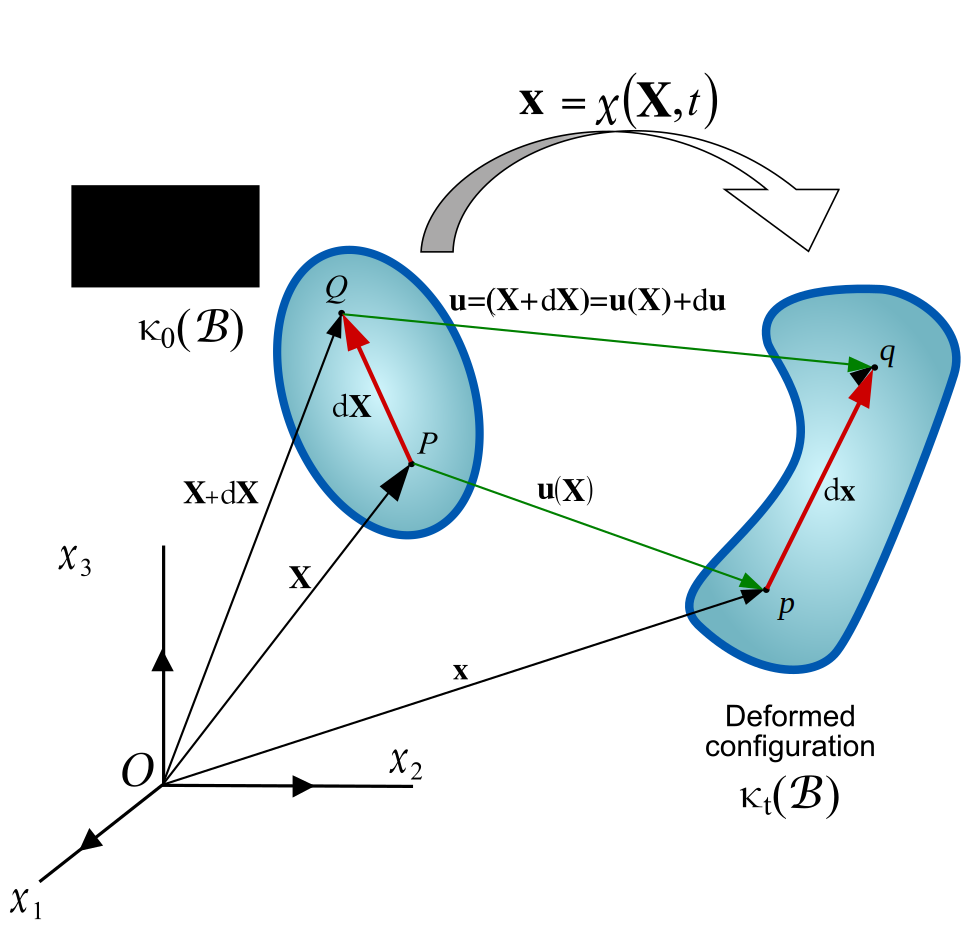
\includegraphics[width=\linewidth]{Pictures/Continuum_body_deformation}
	\end{column}
	%
	\hfill
	%
	\begin{column}{.6\textwidth}
		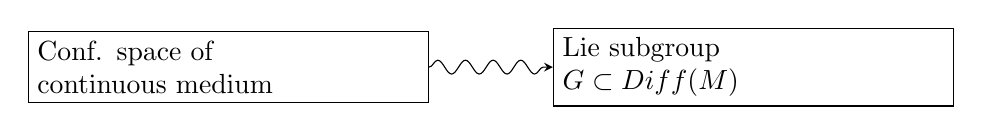
\begin{tikzpicture}[
			text width=0.4\linewidth,
			node distance=0.55\linewidth,
			]
			\node [rectangle,draw] (lhs) {Conf. space of\\ continuous medium};
			\node [rectangle,draw,right of=lhs] (rhs) {Lie subgroup \\$G \subset Diff(M)$};
			\draw[-stealth,decorate,decoration={snake}] (lhs) -- (rhs);
		\end{tikzpicture}

		Examples:
		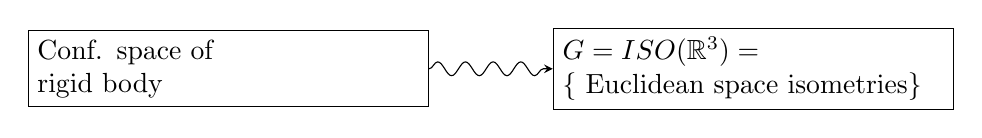
\begin{tikzpicture}[
			text width=0.4\linewidth,
			node distance=0.55\linewidth,
			]
			\node [rectangle,draw] (lhs) {Conf. space of\\ rigid body};
			\node [rectangle,draw,right of=lhs] (rhs) {$G=ISO(\mathbb{R}^3)=$\\ $\{$
				Euclidean space isometries$\}$};
			\draw[-stealth,decorate,decoration={snake}] (lhs) -- (rhs);
		\end{tikzpicture}
		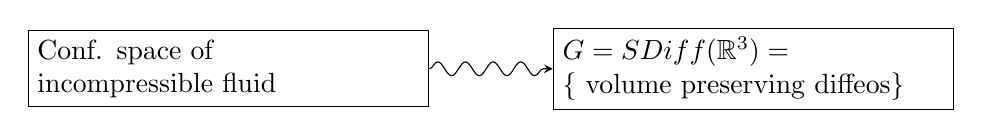
\begin{tikzpicture}[
			text width=0.4\linewidth,
			node distance=0.55\linewidth,
			]
			\node [rectangle,draw] (lhs) {Conf. space of\\ incompressible fluid};
			\node [rectangle,draw,right of=lhs] (rhs) {$G= SDiff(\mathbb{R}^3)=$\\ $\{$
				volume preserving diffeos$\}$};
			\draw[-stealth,decorate,decoration={snake}] (lhs) -- (rhs);
		\end{tikzpicture}
	\end{column}%
	\end{columns}
	\pause
  	\begin{propblock}[$(\mathbb{R}^3,\nu = dx\wedge dy\wedge dz)$ is 2-plectic]
  		\begin{itemize}
  			\item \emph{(Easy proof)} $\quad \iota_v \nu = \frac{1}{2}\epsilon_{i j k} v^i dx^j \wedge dx^k = 0 \; \Leftrightarrow \; v=0 $;
  			\item \emph{(Conceptual proof)} $\quad \alpha^{(1)} = \ast \circ \flat$ is invertible.
  		\end{itemize}
  	\end{propblock}
%		\begin{claimblock} Any oriented manifold is multisymplectic w.r.t. the volume form. \end{claimblock}

		\pause
		 	Consider a subalgebra of the infinitesimal action of $SDiff(\mathbb{R}^3)$:
		  	\begin{displaymath}
		  		\mathfrak{g} = sdiff_0(M) = \lbrace  X \in \mathfrak{X} \quad\vert\quad div X = 0, \textrm{\emph{ rapidly vanishing at }}\infty \rbrace
		  	\end{displaymath}
		  	\centering \alert{(Infinite dimensional Lie algebra!)}
  
  \end{frame}
  \note[itemize]{
	%\item  Now we are ready to get to the real business. Namely, give an explicitly construction of a HCMM related to hydrodynamics.
	\item We are working in the setting of \emph{geometric continuum mechanics} .\\
		Recall that the configuration space of a continuum object is encoded via diffeomorphisms. In the case of an incompressible fluid is encoded via volume-preserving diffeomorphisms.
	\item (Configution space is the set of spatial displacement of a mechanical systems. These are different from the \emph{physical states}.
	\item Such manifolds are infinite dimensional. Particular caution has to be taken when defying in what sense they are smooth.
	\item However, what really pertains to the construction of a moment map is the infinitesimal action, i.e. the Lie algebra. In our case, the infinitesimal action to be considered is via divergence-free vector fields.
	\item (Notation): In the following M will be the 3 dimensional Euclidean Space.
	\item The key, but trivial, observation is that the standard volume form on the euclidean space is a multisymplectic form.
	\item In the following, we will see that the standard Riemannian structure takes a role in our construction. 
	That the reason to show also a "conceptual proof".
	\item Notation: $\ast = $ and $\sharp = $ are respectively the Hodge operator and the Riemmanian sharp operator pertaining to the standard metric in $\mathbb{R}^3$.	
  }
%------------------------------------------------------------------------------------------------


%------------------------------------------------------------------------------------------------
  \subsection{Explicit Construction of the HCMM}
  \begin{frame}{Hydrodynamical homotopy co-momentum map}
  	\begin{claimblock}
  		Explicit construction of an HCMM for $SDiff_0 \circlearrowright (\mathbb{R}^3,\nu)$
  	\end{claimblock}
	\begin{columns}
		\begin{column}[c]{.5\linewidth}
		  	\begin{itemize}
		  		\item The observables are  $$L= \Omega^1_{\textrm{ham}}(\mathbb{R}^3)\oplus\Omega^0(\mathbb{R}^3)$$
		  		\item HCMM consists of a pair of functions:
					\begin{align*}
						f_1 &\colon \mathfrak{g} \rightarrow \Omega^1_{\textrm{ham}}(\mathbb{R}^3) \\
						f_2 &\colon \mathfrak{g}\wedge\mathfrak{g} \rightarrow C^\infty(\mathbb{R}^3)
					\end{align*}	
		  	\end{itemize}
		\end{column}	
	  	\hfill  	
		\begin{column}[c]{.5\linewidth}
  		\includestandalone[width=\textwidth]{Pictures/Figure_Euclid_Trigger}
 	 	\end{column}
 	 \end{columns}
 	\begin{columns}
		\begin{column}[c]{.8\linewidth}
		 	 \begin{itemize}
				\item Satisfying the following system:
					\begin{displaymath}
						\begin{cases}
							\textrm{d} f_1(\xi) = \iota_\xi \nu = -\alpha^1(\xi) \\
							\textrm{d} f_2(\xi_1 \wedge \xi_2) = f_1\left([\xi_1,\xi_2]\right) - \iota_{\xi_2}\iota_{\xi_1} \nu 
							 := \mu_2(\xi_1,\xi_2)\\
							f_2\left(\partial \xi_1 \wedge \xi_2 \wedge \xi_3 \right) = \iota_{\xi_3}\iota_{\xi_2}\iota_{\xi_1} \nu
						\end{cases}
					\end{displaymath}
		 	 \end{itemize}
 	 	\end{column}
		\begin{column}[c]{.2\linewidth}
 	 	\end{column}
 	 \end{columns}
  \end{frame}
	\note[itemize]{
		\item (Regarding the diagram)
		\item On the left there is the part of the Chevalley-Eilemberg complex that interact with the L-$\infty$ algebra of observables.
		\item On the right there is the whole de Rham complex of the manifold $M=\mathbb{R}^3$.
		\item Even if only $\Omega^1$ and $\Omega^0$ take part in the definition of a $HCMM$, the Riemmanian structure determine a correspondence with the rest of the de Rham complex.
		\item In order to give an HCMM for this action is necessary to give a solution of the system of 3 equations below.
		\item Recall: $ 	\ast: \Omega^k \rightarrow \Omega^{n-k}$ where $\ast \sigma$ is defined as the unique form such
		 that $ \omega \wedge \ast \sigma = \nu \lbrace \omega, \sigma \rbrace$ where 
		 $\langle,\rangle$ is the inner product on forms induced by the metric. 
	}  
%---------------------------------------------------------------------------------------------------------------------------------------------------


%--------------------------------------------------------------------------------------------------------------------------------------------------- 
  \begin{frame}[t]{Explicit Construction of the HCMM}
		\begin{enumerate}
			\item<1-> Fix $\vec{b} \in \mathfrak{g}$ and define $f_1(b) := -\vec{A}^\flat$.\\ 
				The first equation is equivalent to solve
				\begin{displaymath}
					\tag{equation of magnetostatic}
					{\rm curl}(\vec{A})=\vec{b}
				\end{displaymath}
				This equation admits a solution 
				\begin{displaymath}
					\tag{Biot-Savart law}
					\vec{A}(r) = \int\frac{\vec{b}\times(\vec{r}-\vec{r}')}{|\vec{r}-\vec{r}'|^3}\textrm{d}r'
				\end{displaymath}							
				\alert {Defined up to a gradient \emph{(gauge freedom)}}. 
			%
			\item<2-> $\mu_2(\xi_1,\xi_2)$ is closed $\forall \xi\in\mathfrak{g}$ $\xRightarrow[\text{lemma}]{\text{Poincar\'e}}$ is exact.\\
				%Hence it is also exact \emph{(Poincar\'e lemma)}.\\
				Take as $f_2(\xi_1,\xi_2)$ a primitive $0$-form, \alert{determined up to a constant $c(\xi_1,\xi_2)$}.
			%
			\item<3-> Third equation is a priori only true up to a constant $c(\xi_1, \xi_2, \xi_3)$.\\
				The constant is zero since $\nu(\xi_1, \xi_2, \xi_3)$ vanishes at infinity and 
				the same is true for $f_2(\partial q)$ upon solving the related Poisson equation
 				\begin{displaymath}
 			 		\Delta f_2(\partial q) = \Delta \nu(\xi_1, \xi_2, \xi_3)			
 				\end{displaymath}
		\end{enumerate}
  \end{frame}
  \note[enumerate]{
  	\item	
  		\begin{itemize}
		  	\item Exploiting the correspondence between tangent fields and 1-form given by the metric is possible to recast the first equation in a simple vector calculus equation containing  the curl.
		  	\item Such equation is the well-known equation of magnetostatic with admits solution by the Biot-Savart law.
		  	\item In the context of hydrodynamic $A$ can be interpreted as a \emph{velocity field} and $b$ as the corresponding vorticity. (See slide for further details)  		
  		\end{itemize}
  	\item In the language of physics, such primitive form is often called "a potential".
  	\item 
  		\begin{itemize}
  			\item (Notation) $q = \xi_1 \wedge \xi_2 \wedge x_3$.
  			\item Last equation tells us that $f_2(\partial q)$ and $ \nu(q)$ differs by a constant. But since both of them vanish at infinity this constant has to be zero.
  			\item The condition of vanishing at infinity has been imposed in order to fulfil the last equation.
  		\end{itemize}
  	\item[$\triangleright$] This construction can be generalized to oriented Riemannian manifolds with further cohomological condition. 
  		See appendix, pag: \ref{frame:RiemannianGeneralization}.
  }
%---------------------------------------------------------------------------------------------------------------------------------------------------


%---------------------------------------------------------------------------------------------------------------------------------------------------
\subsection{Hydrodynamics interpretation}
\begin{frame}[fragile]{Hydrodynamics interpretation}
		Consider the loop spaces $L{\mathbb R}^3$,\\
		%
		\begin{propblock}[HCMM for $G\circlearrowright(\mathbb{R}^3,\nu)$ induces \\an ordinary co-mo.map for $G\circlearrowright (LS,\nu^{\ell})$]
			The HCMM $f \colon \mathfrak{g} \to L_{\infty}(\mathbb{R}^3,\nu)$ previously given
			\emph{transgresses}	 to
			\begin{displaymath}%\tag{Arnol'd-Marsden-Weinstein\\ hydrodynamical co-momentum map}
				\begin{tikzcd}[column sep= small,row sep=0ex]
					\lambda \colon& \mathfrak{g}	\arrow[r]& C^\infty(LS) \\
					& {\mathbf b}	\arrow[r, mapsto]& \displaystyle \lambda_b(\textvisiblespace) =-\oint_{\textvisiblespace} A^\flat = - \oint_{\textvisiblespace} f_1({\mathbf b}) 
					%	\quad \forall \gamma \in LS		
				\end{tikzcd}	
			\end{displaymath}
			that is a  moment map for the induced action $G$ on the pre-symplectic loop space $(LM,\nu^{\ell})$. (Smooth space in the sense of Brylinski)
		\end{propblock}
		\begin{itemize}
			\item $\lambda$ corresponds to \emph{Arnol'd-Marsden-Weinstein hydrodynamical co-momentum map}  defined on $\infty$-dim. manifolds.
			\item<2-> $\Lambda = \left\lbrace \lambda_{\mathbf b} \right\rbrace_{{\mathbf b}\in\mathfrak{g}}$ is, up to sign, the {\it Rasetti-Regge current algebra}
			\item<3-> There is a naturally defined {\it Poisson brackets} on $\Lambda$:
				\begin{displaymath}
					\{ f_1({\mathbf b}), f_1({\mathbf c}) \} (\cdot):= \iota_{\mathbf c} \iota_{\mathbf b} \nu (\cdot)=
						\nu({\mathbf b}, {\mathbf c}, \cdot) = f_1([{\mathbf b},{\mathbf c}])
					-df_2 ({\mathbf b} \wedge {\mathbf c})
				\end{displaymath}
				\centering\footnotesize(Note: $\lambda$ is (infinitesimally) $G$-equivariant, i.e. $	\{\lambda_{\mathbf b}, \lambda_{\mathbf c} \} = \lambda_{[{\mathbf b}, {\mathbf c}]}$)
		\end{itemize}

    
\end{frame}
\note[itemize]{
  	\item[ ] \textbf{How all of this is relevant in Hydrodynamics?}
  	\item The loop space is the manifold, in the sense of Brylinsky, consisting of all smooth loops in ${\mathbb R}^3$.
  	\item Transgression can be seen as a pull-back along the evaluation map 
  		$${\rm ev}: L{\mathbb R}^3 \times {\mathbb R} \ni (\gamma, t) \mapsto \gamma(t) \in {\mathbb R}^3$$
  		  	For further details see appendix, pag: \ref{frame:LoopSpacesTransgression}.
  	\item Note that the (RR) current pertaining to ${\mathbf b} \in {\mathfrak g}$  is independent of the choice of $B$.
  			See appendix, pag: \ref{frame:RRcurrents} for other informations on this concept or \cite{Rasetti1975},\cite{Penna1992} for a deeper account.
  	\item In \cite{Callies2016} is proved a general result asserting that, roughly speaking,
			homotopy co-momentum maps transgress to homotopy co-momentum maps on loop (and even mapping) spaces. Further details in appendix, pag: \ref{frame:TransgressionHCMM}.
	\item Actually, the ansatz for $f_1$ term in the previous construction has been precisely motivated by this phenomenon. 
}
%------------------------------------------------------------------------------------------------

%------------------------------------------------------------------------------------------------
\begin{frame}{Non Equivariance} 
	%
 	\begin{columns}
		\begin{column}[c]{.5\linewidth}	
			\begin{defblock}[$G$-equivariant HCMM]
				$f_i\colon \Lambda^i\mathfrak g\to \Omega^{n-i}(M)$ \\ 
				Ad(G)-equivariant $ \forall i\in\{1,...,n\}$.
			\end{defblock}		
		\end{column}
		\begin{column}[c]{.5\linewidth}	
			\begin{defblock}[$\mathfrak{g}$-equivariant HCMM]
				$\mathcal{L}_{v_x}(f_i(q))=f_i([x,q])$ \\
				\phantom{\hspace{2cm}}$\forall q\in \Lambda^{i}\mathfrak g , \: x\in \mathfrak g$\\
				\footnotesize{Where $[x,\cdot]$ is $ad(x)$ acting  on $\Lambda^\bullet \mathfrak g$}
				%$f_i\colon \Lambda^i\mathfrak g\to \Omega^{n-i}(M)$
			\end{defblock}		
		\end{column}
	\end{columns}
	\pause
	\vfill
	\begin{propblock}[$(f)$ is not $\mathfrak{g}$-equivariant]
		\underline{Proof:} 
		\footnotesize
		Consider in particular $\xi = \vec{b} \in \mathfrak{g}$, one should check 
		\begin{displaymath}
			\begin{split}
				0 = f_1\left( [\xi, \vec{b}] \right)
				\stackrel{?}{=}
				%=?=
				{\mathcal L}_{\xi} f_1({\vec{b}})  = -{\mathcal L}_{\xi} \vec{A}^\flat &=
					- d \iota_\xi \vec{A}^\flat = - d \langle \vec{A}, \vec{b} \rangle_g
				\qquad \forall \xi \in \mathfrak{g} \\
						\text{(vanishing at infinity condition)} &\Rightarrow \langle \vec{A}, \vec{b} \rangle_g = 0
			\end{split}
%		\begin{split}
%					f_1\left( [\xi, \vec{b}] \right) &= 0 \\
%					 ( \forall \xi\in \mathfrak{g}) \quad \parallel ? & \qquad\\
%					{\mathcal L}_{\xi} f_1({\vec{b}})  &= -{\mathcal L}_{\xi} \vec{A}^\flat =
%					- d \iota_\xi \vec{A}^\flat = - d \langle \vec{A}, \vec{b} \rangle_g
%		\end{split}		
		\end{displaymath}
		%
	 	\begin{columns}
			\begin{column}[c]{.7\linewidth}
				(By contradiction), consider $\vec{b}\in\mathfrak{g}$ supported on two linked flux tubes
				$(\text{supp}(\vec{b}) = \Gamma_1 \cup \Gamma_2)$, one gets
		\begin{displaymath}
			\int \langle \vec{A}, \vec{b} \rangle_g = 2 \mathbf{n} \Phi_1 \Phi_2 
			\qquad \text{with} \quad 
			\Phi_i = \int_{S_i} \hat{n} \cdot \vec{b}\, d\sigma
		\end{displaymath}
		where $n \in \mathbb{N}$ \emph{(Gauss linking number)}, results
		$$\mathbf{n} \neq 0 \qquad \Rightarrow \quad {\mathcal L}_{\xi} f_1({\vec{b}}) \neq 0  \quad \Rightarrow \quad\text{\bomb}$$ 
			\end{column}
			\begin{column}[c]{.45\linewidth}	
				\includegraphics[width=0.9\linewidth]{Pictures/VortexLink}
			\end{column}
		\end{columns}	
	\end{propblock}

		
\end{frame}
\note[itemize]{
    \item We may also naturally ask the question whether the above map $(f)$ is (infinitesimally) {\it G-equivariant}, in the sense of \cite{RWZ}.
    \item In the symplectic case, $G$ connected implies $G$-equivariance. This does not hold true in the multisymplectic case. (ask Leyli!)
    \item In the proof, if $\vec{A}$ is the velocity field of the fluid, $\vec{b}$ is the associated vorticity, the quantity $\langle \vec{A}, \vec{b} \rangle_g$ is called \emph{Helicity}, see below (pag. \ref{Frame:VortexLinks}) for further details.
    \item The proof is by contradiction by exhibiting an example of solenoidal field $\vec{b} = \text{curl}(\vec{A})$ with non vanishing helicity, i.e. not satisfying the condition.\\
    Namely, consider a solenoidal field compactly supported  on a domain $D$ consisting in two disjoint, unknotted but linked closed tubes.
    \item  See \cite{Moffatt-Ricca92} for further elucidation on the non vanishing of the Helicity in the cosidered case.
    Notice that the argument does not depend on the choice of	$\vec{A}$ pertaining to the fixed $\vec{b}$.
    \item The lack of $G$-equivariance is not surprising, since our construction involves Riemannian geometric features.	
}
%------------------------------------------------------------------------------------------------

\end{document}
%-------------------------------------------------------------------------------------------------------------------------------------
\begin{frame}{going beyond fluid}
	\begin{columns}
		\begin{column}[T]{0.5\textwidth}
	        \centering
	        \resizebox {0.85\columnwidth} {!} {
				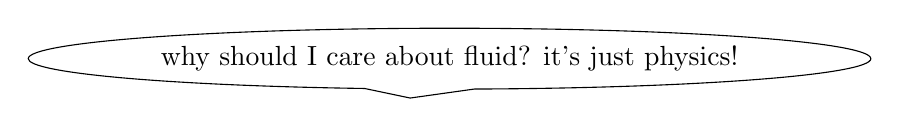
\begin{tikzpicture}
					\node[ellipse callout,draw, callout absolute pointer={(0.5,0)}]   at (1,0.5)
					{why should I care about fluid? it's just physics!};
				\end{tikzpicture}
			}
		\end{column}
		\begin{column}[T]{0.5\textwidth} 
	        \centering
	        \resizebox {0.85\columnwidth} {!} {
				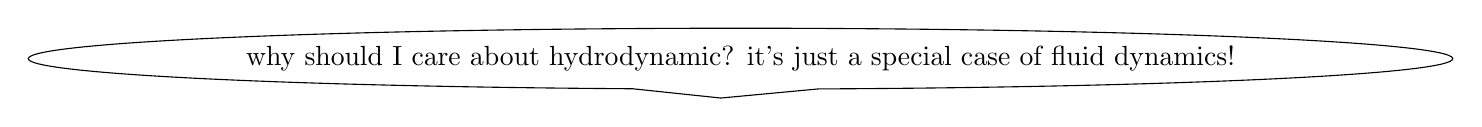
\begin{tikzpicture}
					\node[ellipse callout,draw, callout absolute pointer={(0.75,0)}]   at (1,0.5)					{why should I care about hydrodynamic? it's just a special case of fluid dynamics!};
				\end{tikzpicture}
			}
		\end{column}
	\end{columns}
	\begin{figure}
		\includegraphics[scale=0.5]{Pictures/purity}
	\end{figure}

  	Comic:
  		mathematician: "why should I care about fluid? it's just physics!\\
  		physicists: "why should I care about hydrodynamic? it's just a special case of fluid dynamics!\\  
  		
  	Concetto filosofico / crackpot:\\
  	Così come si usano le geodetiche per sondare le varietà riemmaniane si può usare il fluido perfetto (esteso in tutta la varietà).\\
  	+++ (vedi talk Spera) si può codificare questo problema comunque come una geodetica!
  	
  	Inoltre:\\
  	Ubiquitus role of the group of orientation preserving diffeomorphisms!
\end{frame}
\note[itemize]{
	\item It's a joke from the point of view of theoretician! It's clear that if you are inclined to application there are endless possibilities!

\url{https://xkcd.com/435/}
}
%-------------------------------------------------------------------------------------------------------------------------------------
  
%------------------------------------------------------------------------------------------------

%------------------------------------------------------------------------------------------------
\section{Knots in Hydrodynamics}
\checkpoint
%+----------------------------------------------------------------------------+
%| SLIDES: Longer presentation on my paper 1805.01696
%| Chapter: multisymplectic geometry and knot theory
%| Author: Antonio miti
%| Event: Visit in Salerno, March 2019
%+----------------------------------------------------------------------------+

%- HandOut Flag -----------------------------------------------------------------------------------------
\newif\ifHandout
	\Handouttrue  %uncomment for the printable version

%- D0cum3nt ----------------------------------------------------------------------------------------------
\documentclass[beamer,10pt]{standalone}


%- Packages ----------------------------------------------------------------------------------------------
\usepackage{verbatim}
\usepackage{appendixnumberbeamer}

\usepackage{amsmath, amssymb}
\usepackage{tikz}
\usetikzlibrary{arrows,shapes,calc}
\usetikzlibrary{shapes.callouts}
\usepackage{tikz-cd}
\usepackage{graphicx, animate}
\usepackage{hyperref}
\usepackage[english]{babel}
\usepackage{csquotes}
\usepackage{stackengine}
\usepackage{fourier} %Danger Sign

\usepackage[mode=buildnew,subpreambles=true]{standalone}



\providecommand{\blank}{\text{\textvisiblespace}}

%--Beamer Style-----------------------------------------------------------------------------------------------
\usetheme{toninus}



%%- WorkAround --------------------------------------------------------------------------------------------------------------
%Standalone with relative path
\providecommand{\includestandalonewithpath}[3][]
{
  \begingroup
  \newcommand{\datapath}{#2}
  \includestandalone[#1]{\datapath/#3}
  \endgroup
}





%---------------------------------------------------------------------------------------------------------------------------------------------------
%- D0cum3nt ----------------------------------------------------------------------------------------------------------------------------------
\begin{document}
%------------------------------------------------------------------------------------------------

%------------------------------------------------------------------------------------------------
\begin{frame}{A connection with Knot theory}\label{Frame:VortexLinks}
 	\centering$\Rightarrow$\emph{The bridge is the \alert{Vortex Dynamics}}$\Leftarrow$

	\begin{columns}
	\begin{column}[T]{.55\linewidth}
		\vspace{1ex}
 		$\bullet$Consider a perfect (incompressible, inviscid) fluid permeating the  whole space $M=\mathbb{R}^3$.\\
 		\pause
 		$\bullet$ $\text{Physical state} \rightsquigarrow u \in sdiff_0(\mathbb{R}^3)$
% 		\begin{displaymath}
% 			\text{physical state} \rightsquigarrow u \in sdiff_0(\mathbb{R}^3)
% 		\end{displaymath}
 		\begin{columns}
 		\begin{column}{.5\linewidth}	
 			\begin{defblock}[Vorticity]
				$\displaystyle \omega := \textrm{curl}(u)$					
 			\end{defblock}
 		\end{column}
  		\begin{column}{.5\linewidth}	
 			\begin{defblock}[Helicity]
				$\displaystyle h = \int_{\mathbb{R}^3} u \cdot \omega  d^3x$		
 			\end{defblock} 		
 		\end{column}
 		\end{columns}
 				%
  		\begin{columns}
 		\begin{column}{.5\linewidth}	
 			\pause
			$\bullet$ Dynamics is ruled by the \emph{Euler equation}:
			\begin{displaymath}
				\frac{\partial \omega}{\partial t} = [\omega, u]				
			\end{displaymath}
 		\end{column}
  		\begin{column}{.5\linewidth}	
			\begin{propblock}[Helicity is conserved]
				$\frac{d}{dt}H = 0$
			\end{propblock}
 		\end{column}
 		\end{columns}
 			\pause
 			\vspace{2ex}
 			$\bullet$
 			Consider $\omega$ localized in a flux loop $\mathcal{L}$.
 			\begin{propblock}[Vortex filaments are preserved]
 				$\text{supp}(\omega(0))\simeq \text{supp}(\omega(t)) \qquad \forall t$
  			\end{propblock}
	\end{column}
	\begin{column}[T]{.40\linewidth}
		\vspace{-1ex}
		\pause
		\begin{figure}[T]
			\caption{Knotted vortex in water  (Klenecker \& Irvine \cite{Kleckner2013})}
			\href{https://www.nature.com/articles/nphys2560}{\includegraphics[width=\linewidth]{Pictures/knottedwatervortex}}
		\end{figure}
			\vspace{-2ex}
			\alert{Such fluid configurations are proved to exist both 
			\underline{theoretically} and \underline{experimentally}!}
	\end{column}
	\end{columns} 
\end{frame}
\note[itemize]{
	\item One of the  the main goal of our paper\cite{Miti2018} is to find an application of this construction in knot theory.
	\item The cornerstone of this idea is to recognize the ubiquitous role of the group of preserving diffeomorphisms. 
	The first step is to notice that conserved quantities can be associated to any fluid configurations (especially knotted ones).
 	\item The gist of the second proposition is that the topology of the support of the vorticity is conserved along the fluid evolution.
 	\item The image on the right represents a fluid configuration with knotted vorticity realized in the laboratory.
}
%------------------------------------------------------------------------------------------------

%-------------------------------------------------------------------------------------------------------------------------------------
\subsection{Basics of Knot theory}
%-------------------------------------------------------------------------------------------------------------------------------------
  \begin{frame}[fragile]{Basics of \emph{knots theory}}
		\begin{columns}
			\begin{column}[T]{.4\linewidth}
				\begin{figure}
					\caption{Reidmeister's move}
				\ifHandout
					\includestandalonewithpath[width=\textwidth,keepaspectratio]{./Pictures}{Figure_trefoil}
				\else
					\includestandalonewithpath[width=\textwidth,keepaspectratio]{./Pictures}{Animation_trefoil}
				\fi
				\end{figure}
			\end{column}
				\hfill
			\begin{column}[T]{.6\linewidth}
				\begin{enumerate}
					\item Knots = compact submanifolds of codimension 2 embedded in $\mathbb{R}^3$
						\begin{defblock}[n-link]
							%Disjoint union is written using \coprod, since it is in fact the coproduct in the category of sets.(\amalg)
							$\gamma: {\displaystyle\coprod_1^n S^1 } \to \mathbb{R}^3 $ embedding.				
						\end{defblock}
					\item studied \emph{modulo "ambient isotopies"}
						\begin{defblock}[Ambient isotopies]
							%Disjoint union is written using \coprod, since it is in fact the coproduct in the category of sets.(\amalg)
							$h : {\displaystyle\coprod_1^n S^1 }\times [0,1] \to \mathbb{R}^3 $ smooth homotopy
							s.t. $\hat{h}(t) : {\displaystyle\coprod_1^n S^1 } \to \mathbb{R}^3$ is an embedding $\forall t$	.				
						\end{defblock}	
					\item Holy grail of knot theory: classify all non equivalent (by ambient isotopies) n-links.
					\item \alert{These classes are invariant w.r.t. volume preserving diffeos.}
				\end{enumerate}
				%			
  	  \end{column}
    \end{columns}
	%
 \end{frame}
\note{
	\begin{itemize}
		\item It is possible to build a bridge between knot theory and multisymplectic geometry exploiting the tight connection between both of them with hydrodynamics.\\
		The cornerstone of this relationship is the ubiquitous role of the group of volume preserving diffeomorphisms.
		\item Knot  theory is not simply an instance of studying the topology of loops but the ambient space takes a significant role"
		\item Studying smooth knots is equivalent to study \href{http://mathworld.wolfram.com/PolygonalKnot.html}{tamed polygonal knots}.
		\item choosing a smooth parametrization is tantamount to fix an orientation of the knot.
	\end{itemize}
}
%-------------------------------------------------------------------------------------------------------------------------------------

%-------------------------------------------------------------------------------------------------------------------------------------
\subsection{Intermezzo: Poincare duals}
%------------------------------------------------------------------------------------------------

%------------------------------------------------------------------------------------------------
\begin{frame}{Recall: De Rham currents}
	On smooth manifolds is possible to mimick the basic definition of distribution using differential forms:
		\begin{defblock}[De Rham k-Currents]
			\begin{displaymath}
				\mathcal{D}_k(M)
				:= 
			\biggr\{\eta: \Omega^k_c(M)\rightarrow \mathbb{R} \; \left\vert \; \text{\stackanchor{(seq.) continuous}{linear functionals}} \right\} 
				\cong
				\left(\Omega^k_c (M) \right)^\ast
			\end{displaymath}
		\end{defblock}
		%
		\vspace{-2.5ex}
		%
  	\onslide<2->{
  	\begin{columns}
		\begin{column}[t]{.5\linewidth}	
			\begin{defblock}[Annihilation set of $T \in \mathcal{D}$]
				Open subset $A \subset M$ s.t. \\ 
				$\langle T, \phi \rangle = 0 \quad \forall \phi 	
				\text{ s.t. } \text{supp}(\phi) \subset A$
			\end{defblock}
		\end{column}
		\begin{column}[t]{.5\linewidth}			
			\begin{defblock}[Support of $T \in \mathcal{D}$]
				$\text{supp}(T)$ = complement of the union of all open annihilation sets of $\eta$
			\end{defblock}
		\end{column}
  	\end{columns}
  	}		
%
  	\onslide<3->{
	  	We have the analogue of \emph{regular distributions}
			\begin{alignat*}{2}
			  D:\Omega^k(M) & \longrightarrow & \mathcal{D}^{n-k}(M) & \\
			  \eta & \longmapsto & D_\eta & \quad:\quad 
			  \langle D_\eta, \text{\textvisiblespace} \rangle = 
			  \int_M \blank \wedge \eta \\
			  \text{d}\sigma& \longmapsto & D_{\text{d}\sigma} & \quad:\quad 
			  \langle D_{\text{d}\sigma}, \blank \rangle = 
			  (-)^{k} \int_M   \text{d}\blank \wedge\sigma
			\end{alignat*}	  	
  	}				
		%
		\vspace{-2.5ex}
		%
  	\onslide<4->{
		\begin{defblock}[De Rham boundary operator]
			\begin{displaymath}
				\partial : \mathcal{D}_k(M) \rightarrow \mathcal{D}_{k-1}(M) \qquad \text{s.t.} \quad
				\langle \partial T, \blank \rangle = (-)^{k} \langle T, \text{d}\blank \rangle
			\end{displaymath}
		\end{defblock}
  	}							
\end{frame}
\note[itemize]{
	\item this is the analogue of the theory of distribution on $\mathbb{R}^n$
	\item Continuity in the sense of distributions means \emph{sequentially continuous} i.e
		If a sequence $\omega_{k}$ of smooth forms, all supported in the same compact set, is such that all derivatives of all their coefficients tend uniformly to 0 when 
		$k$ tends to infinity, then $T(\omega_{k})$ tends to 0.
	\item $\Omega^k_c(M)$ stands for compact supported k-forms.
	\item Recall the definition of \emph{support} of a differential form
		$$
			\text{supp}(\omega) := \overline{\lbrace p \in M \; \vert \: \omega_p = 0 \rbrace}
		$$
	\item from the definition of regular distribution we obtain the definition of boundary operator.	
	\item De Rham distributions build up a chain complex which is dual (modulo a sign) to the de Rham co-chain complex.
}
%------------------------------------------------------------------------------------------------



%------------------------------------------------------------------------------------------------
\begin{frame}{Recall:Poincaré duals}
	Given a compact, oriented embedded k-dim submanifold $\Sigma$ of $M$ (n-dim)
	\begin{displaymath}
		\left( i : 	\Sigma \hookrightarrow M \right) \in \text{Emb}_c(k)
	\end{displaymath}		
	you can associate a compactly supported \emph{DeRham current} $D_\Sigma$ defined as
	\begin{displaymath}
		\langle D_\Sigma, \omega\rangle = \int_\Sigma i^\ast (\omega) \qquad 
		\forall \omega \in \Omega^k
	\end{displaymath}
		%
		\vspace{-2.5ex}
		%
	\onslide<2->{
  	\begin{columns}
		\begin{column}[c]{.5\linewidth}	
			\begin{claimblock}
				$\partial D_\Sigma = (-)^{k-1} D_{\partial \Sigma}$ 
			\end{claimblock}
		\end{column}
		\begin{column}[c]{.5\linewidth}			
			\begin{claimblock}
				$ D_{\Sigma_1} \wedge D_{\Sigma_2} = D_{\Sigma_1 \cap \Sigma_2}$
			\end{claimblock}
		\end{column}
  	\end{columns}
  }		
	%
	\onslide<3->{
		\begin{table}[]
		\begin{tabular}{lll}
			Analogue of the Dirac delta function localized on $\Sigma$ & $\Rightarrow$ & 
			\alert{\danger non regular \danger}
		\end{tabular}
		\end{table}

		We're interested in a \emph{regular approximation} (regularization)
		\begin{defblock}[a (smooth) Poincaré dual of $\Sigma$]
		 $\eta_\Sigma \in \Omega^k$ supported on a tubular neighbourhood $T$ of $\Sigma$ s.t.
		 \begin{displaymath}
				\langle D_{\eta_\Sigma},\omega\rangle \equiv \int_M \omega \wedge \eta_\Sigma =
				\int_T i^\ast \omega \sim 
				\langle D_{\Sigma},\omega\rangle 
		 \end{displaymath}
		\end{defblock}		
		  	\centering \alert{\danger \; ( Not unique! ) \; \danger}

  }		
\end{frame}
\note[itemize]{
	\footnotesize
	\item $\forall$ compact submanifold (dim=k) of $M$ (dim= n) one can associates a unique
	 de Rham current. 
	They can be understood as \emph{generalized} differential $(n-k)$-forms concentrated on $\Sigma$.
	This is the analogue of the Dirac delta function localized on $\Sigma$.
	\item Usual definition of Poincar\'e dual (in algebraic topology) is different:
	\\
		%\begin{defblock}[Poincaré dual of $\Sigma$]
			Unique $[\eta_\Sigma ] \in H^{n-k}_c(M)$ s.t.
			\begin{displaymath}
				\int_\Sigma i^\ast \omega = \int_M \omega \wedge \eta_\Sigma \qquad \forall [\omega] \in H^k(M)
			\end{displaymath}
		%\end{defblock}
		More conceptually, Poincaré duals can be seen as \emph{Thom Classes}.
	
	\item Proof of claim 1 is direct:
		\begin{displaymath}
			(-)^{k-1} \langle \partial D_\Sigma , \omega \rangle = 
			\langle D_\Sigma, d\omega\rangle =
			\int_\Sigma i^\ast d \omega = 
			 \int_\Sigma d i^\ast \omega = 
			 \int_{\partial \Sigma} i^\ast \omega =
			\langle D_{\partial \Sigma}, \omega \rangle
		\end{displaymath}
	\item Claim 2 is better understood with smooth Poincarè duals:
		\begin{displaymath}
			\text{supp}(\eta_1 \wedge \eta_2) \subset
			\text{supp}(\eta_1) \cap \text{supp}(\eta_2) \subset
			T_{\Sigma_1 \cap \Sigma_2} \quad\Rightarrow\quad
			\eta_1 \wedge \eta_2 = \eta_{\Sigma_1 \cap \Sigma_2}	
		\end{displaymath}				
		An example: 
		Take as $\Sigma_1$ the $z$-line in $\mathbb{R}^3$, $\eta_1 = \delta_{\{x=y=0\}}	dx \wedge dy$, and as $\Sigma_2$ the $xy$-plane, $\eta_2= \delta_{\{z=0\}} dz$.
		You get $\eta_1 \wedge \eta_2 = \delta_{\{x=y=z=0\}} dx \wedge dy \wedge dz = \eta_{\Sigma_1 \cap \Sigma_2}$
}
%------------------------------------------------------------------------------------------------




%-------------------------------------------------------------------------------------------------------------------------------------
\subsection{Invariant quantities related to knotted configurations}
%------------------------------------------------------------------------------------------------
\begin{frame}{Hamiltonian forms related to a n-link}

		
  	\onslide<1->{
  	\begin{columns}
		\begin{column}[c]{.7\linewidth}	
				Let $ L = \cup_{i=1}^n L_i$ be an oriented link in ${\mathbb R}^3$ 
				\\(components $L_i$, $i=1,\dots,n$ required to be  {\it trivial} knots)	
		\end{column}
		\begin{column}[c]{.25\linewidth}	
			\centering{
			\includegraphics[width=0.75\linewidth]{Pictures/Whiteheadlink}
			}
		\end{column}
  	\end{columns}
  	}
		%
  	\onslide<2->{
  	\begin{columns}
		\begin{column}[t]{.5\linewidth}	
			\begin{defblock}[Vorticity 2-form]
				$$
				\omega_{L} := \sum_{i=1}^n \omega_{L_i}, \qquad d\omega_L = 0
				$$
				($\omega_{ L_i}$ = Poincar\'e dual associated to $L_i$)
			\end{defblock}
		\end{column}
		\begin{column}[t]{.5\linewidth}	
			\begin{defblock}[Velocity 1-form]
				$$
 					v_{ L} = \sum_{i=1}^n v_{L_i}, \qquad \qquad  dv_{L} = \omega_{ L}
				$$
				($v_{L_i} := \omega_{{\mathfrak a}_i}$ = Poincar\'e dual  of a disc ${\mathfrak a}_i$ 
				bounded by 	$L_i$ \footnotesize{(Seifert surface)}) 
			\end{defblock}						
		\end{column}
  	\end{columns}
  	}
  	%
  	\begin{columns}
		\begin{column}[t]{.3\linewidth}	
  		\onslide<2->{
  			\center
  			\vspace{-4ex}
				\includegraphics[width=0.6\linewidth]{Pictures/tubes}
	  	}			
		\end{column}
		\begin{column}[t]{.7\linewidth}	
  	\onslide<3->{
			\begin{propblock}[$v_{L}$ is a {\it Hamiltonian 1-form}]
				For each component $L_i$, the Hamiltonian vector field $\xi_{L_i}$ of 
				$v_{L_i}$ is $-\alpha^{-1}(\omega_{L_i})$.
				\\
				Explicitly, one has 
				\begin{displaymath}
					dv_L + \sum_{i=1}^n\iota_{\xi_{L_i}} \nu = 0 				
				\end{displaymath}
			\end{propblock}  	
  	}				
		\end{column}
  	\end{columns}
\end{frame}
\note[itemize]{
	\item $\omega_{ L_i}$ denote the Poincar\'e (or Thom) dual (class) associated to $L_i$: they are 2-forms localized in a 
 cross-section of a  suitable tubular neighbourhood $T_i$ around $L_i$ - with total fibre integral equal to one, or, as currents, 2-forms which are $\delta$-like on $L_i$
 
	\item $v_{L_i} := \omega_{{\mathfrak a}_i}$ is the Poincar\'e dual (class) of a disc ${\mathfrak a}_i$ bounding
$L_i$ (a Seifert surface for the trivial knot $L_i$). Precisely:
$$
\partial {\mathfrak a}_i = L_i, \qquad \qquad dv_{L_i} = d\omega_{{\mathfrak a}_i} = \omega_{L_i} = \omega_{\partial {\mathfrak a}_i},
$$
	\item
		Velocity 1-forms $v_i$ correspond (upon approximation of the associated Euler equation) to the so-called LIA (Linear Induction Approximation) or  {\it binormal evolution}
		of the ``vortex ring" $L_i$ (``orthogonal" to the discs ${\mathfrak a}_i$.
		
	\item Everything is up to choices of tubular neighbourhoods, Seifert surface and specific Poincar\'e dual.


}
%------------------------------------------------------------------------------------------------


%------------------------------------------------------------------------------------------------
\begin{frame}{Relation with Gauss linking number}
		%
		\vspace{-2.5ex}
		%
  	\begin{columns}
		\begin{column}[t]{.5\linewidth}	
			\begin{defblock}[Chern-Simons 3-form]
				$$
					CS({L}) :=  v_{L} \wedge  \omega_{ L} 
				$$
			\end{defblock}
		\end{column}
		\begin{column}[t]{.5\linewidth}	
			\begin{defblock}[Helicity]
				$$
 					{\mathcal H}(L) = \int_{\mathbb{R}^3} CS({L})
				$$
			\end{defblock}						
		\end{column}
  	\end{columns}
	\pause
	\begin{propblock}[
		Choosing a parametrization $\mathbf{r}_i$ (in standard coordinates) for each $L_i$ 
		\begin{displaymath}
			{\mathcal H}(L)  = 
			\sum_{i,j=1}^n
			\,\frac{1}{4\pi}
			\oint_{\gamma_i}\oint_{\gamma_j}
			\frac{\mathbf{r}_i - \mathbf{r}_j}{|\mathbf{r}_i - \mathbf{r}_j|^3}
			\cdot (d\mathbf{r}_i \times d\mathbf{r}_j) =
			\sum_{i,j=1}^n \ell(i,j)
		\end{displaymath}
			$\bullet$ $\ell(i,j) = \ell(j,i)$ : Gauss linking number of components $L_i$ and $L_j$ if $i\neq j$\\
			$\bullet$ $\ell(j,j)$ : {\it framing} of $L_j$\\ 
			\phantom{-------}\footnotesize{ (i.e. $\ell(L_j, L_j^{\prime})$ with $L_j^{\prime}$ being a section of the normal bundle of $L_j$.)}\normalsize

		]
	\pause
  	\begin{columns}
		\begin{column}[c]{.7\linewidth}	
		\underline{Sketch}: Cosider a Hopf Link
			\begin{displaymath}
				L(C,C') = \eta_C \wedge \eta_{\Sigma'} + \eta_{C'} \wedge \eta_\Sigma =
				\eta_{P'} + \eta_{P}
			\end{displaymath}
		\end{column}
		\begin{column}[c]{.25\linewidth}	
			\centering{
			\includegraphics[width=0.75\linewidth]{Pictures/GaussLink}
			}
		\end{column}
  	\end{columns}
			Therefore $\int L(C,C') = \ell(C,C')$ is counting the times that a knot cross another Seifert surface with sign given by the orientation.
		\end{propblock}
		
\end{frame}
\note[itemize]{
	\item Our previous construction is heavily dependent on a lot of choices 
	but we end up with a quantity that only depends on the starting n-link.
	\item ${\mathcal H}(L)$ is invariant under ambient isotopies.\\
	However, non ambient isotopic links do not necessarily yield different linking numbers
	(it is not an universal invariant!).
  	\begin{columns}
		\begin{column}[c]{.5\linewidth}	
			\centering{
			\includegraphics[width=0.5\linewidth]{Pictures/UnknotsGauss}
			}
		\end{column}
		\begin{column}[c]{.5\linewidth}	
			\centering{
			\includegraphics[width=0.35\linewidth]{Pictures/WhiteheadGauss}
			}
		\end{column}
  	\end{columns}	
	\item
		\begin{displaymath}
	\begin{split}
		\text{link}(\gamma_1,\gamma_2) &=\,\frac{1}{4\pi}
		\oint_{\gamma_1}\oint_{\gamma_2}
		\frac{\mathbf{r}_1 - \mathbf{r}_2}{|\mathbf{r}_1 - \mathbf{r}_2|^3}
		\cdot (d\mathbf{r}_1 \times d\mathbf{r}_2)\\[4pt]
		 &= \frac{1}{4\pi}\int_{S^1 \times S^1} \frac{\text{det}(\dot{\gamma_1}(s),
	 \dot{\gamma_2}(t),\gamma_1(s)-\gamma_2(t))}{|\gamma_1(s)-\gamma_2(t)|^3}\, ds \, dt
	\end{split}
	\end{displaymath}			
}
%------------------------------------------------------------------------------------------------

%-------------------------------------------------------------------------------------------------------------------------------------
\subsection{Higher order link invariants}
%------------------------------------------------------------------------------------------------

%------------------------------------------------------------------------------------------------
\begin{frame}{Cohomological interpretation of the linking number}
		\vspace{2ex}
  	\begin{columns}
		\begin{column}[c]{.75\linewidth}	
			$\bullet$ Choose a pair of linked knots (part of a more complex link).
			Define
			$$ \Xi_{1 2} := - v_{L_1} \wedge v_{L_2} \in \Omega^2(\mathbb{R}^3)$$
			you get:
			\begin{displaymath}
				\begin{split}
				d \Xi_{1 2} =& -\omega_1 \wedge v_2 + v_1 \wedge \omega_2 = CS({L_1\cup L_2}) - 
				\text{"\stackanchor{self}{linking}"}
				\\
				&\Rightarrow \int d \Xi_{1 2} = \ell(1,2)
				\end{split}
			\end{displaymath}		
		\end{column}
		\begin{column}[c]{.20\linewidth}	
			\centering{
			\includegraphics[width=\linewidth]{Pictures/WhiteheadGauss}
			}
		\end{column}
  	\end{columns}	
	\pause	
	\vspace{1ex}
	$\bullet$ While $\Xi_{1 2}$ is not uniquely defined,it determines an unique class in the \emph{cohomology of the link}
	(independent of the choices)
	\begin{displaymath}
		\langle L_1, L_2 	\rangle := 
		\left[\Xi_{1 2}\bigg\rvert_{S^3\setminus L} \right] \in H^2(S^3\setminus L)
	\end{displaymath}
	\pause
	\vspace{-2ex}
  	\begin{columns}
		\begin{column}[c]{.72\linewidth}	
			\begin{propblock}[$\ell(1,2)= 0 \Leftrightarrow \langle L_1, L_2 \rangle = 0$]
				\vspace{-4ex}
				\begin{displaymath}
				\begin{split}
					l(1,2)=0 \quad&\Leftrightarrow\quad d \Xi_{1 2} = 0 \in \Omega^2(\mathbb{R}^3)\\
					\text{"Poincar\'e lemma"}	
					\quad&\Rightarrow\quad \exists v_{1 2} \;:\; d v_{1 2} = \Xi_{ 1 2}	\\
					[ \Xi_{1 2} ] = 0 \in H^2(\mathbb{R}^3) \quad&\Rightarrow\quad
					\left[\Xi_{1 2}\bigg\rvert_{S^3\setminus L} \right] = 0 \in H^2(S^3\setminus L)
				\end{split}
				\end{displaymath}		
			\end{propblock}
		\end{column}
		\begin{column}[c]{.3\linewidth}	
	  	\begin{asideblock}[Cohomology groups of a n-Link]%Shades of...
  			\begin{table}[] % http://tablesgenerator.com/
					\begin{tabular}{l}
						$H^0 (S^3 \setminus L) \cong {\mathbb R}$ \\
						$H^1 (S^3 \setminus L) \cong {\mathbb R}^{n}$ \\
						$H^2 (S^3 \setminus L) \cong {\mathbb R}^{n-1}$ \\
						$H^3 (S^3 \setminus L) \cong 0$
					\end{tabular}
				\end{table}
	  	\end{asideblock}
		\end{column}
  	\end{columns}			



	

\end{frame}
\note[itemize]{
	\item The cohomology of a n-link is the de Rham cohomology of $S^3 \setminus L$, 
	where $S^3$ has to be understood as the compactification of the Euclidean space
	\item Being $\Xi_{1 2}$ closed follows from the fact that 
	$\text{supp}(d \Xi_{1 2}) \subseteq L$ \\
	Similarly, you get that all the velocity 1-forms $v_i$ are closed.
	The cohomology classes of these forms, one for each component of the link, 
	are precisely the generators of $H^1 (S^3 \setminus L)$.
	\item Why such a class is called a number? 
	The name follows from the simplest case of $n=2$.
	\item \underline{Upshot:} we can associate to any pair of knots in a link a  cohomology class.
}
%------------------------------------------------------------------------------------------------

%------------------------------------------------------------------------------------------------
\begin{frame}{Higher order linking numbers}
	\begin{itemize}
		\item[•] Take a link with 3 or more components
		\item[•] 	assume all ordinary mutual linking numbers vanish: $\langle L_i, L_j \rangle =0$
		\item[•] Out of the primitives obtained in the previous proposition you can manufacture another closed 2-form
	\end{itemize}
		\vspace{-2ex}
  	\begin{columns}
		\begin{column}[c]{.5\linewidth}	
			\begin{defblock}[Massey product]
				$\Xi_{1 2 3} = - v_1 \wedge v_{2 3} - v_{1 2} \wedge v_3 
				\in \Omega^2(\mathbb{R^3})$
			\end{defblock}
		\end{column}
		\begin{column}[c]{.5\linewidth}	
			\begin{defblock}[Third order linking number (class)]
				$\langle L_1, L_2, L_3 \rangle := 
				\left[\Xi_{1 2 3}\bigg\rvert_{S^3\setminus L} \right]
				\in H^2(S^3\setminus L)$
			\end{defblock}
		\end{column}
  	\end{columns}			
  	\pause
	The procedure can be iterated (obstructed by the non vanishing of a higher linking number) yielding a hierarchy of pairs
	\begin{displaymath}
		\Xi_I \in \Omega^2 \qquad v_I \in \Omega^1
	\end{displaymath}
	\center
	\footnotesize{(I = multi index constructed out of the set $\{1,\ldots,n\}$ of the $n$-link components)}\normalsize 

	\pause 	\center 	\textbf{-- Applications --}
  	\begin{columns}
		\begin{column}[c]{.45\linewidth}
			Distinguish different links with same (vanishing) Gauss linking number	
			\center
			\begin{tikzpicture}
			\node[inner sep=0pt] (A) at (0,0)
			    {\includegraphics[width=.4\textwidth]{Pictures/UnknotsGauss}};
			\node[inner sep=0pt] (B) at (3,0)
			    {\includegraphics[width=.4\textwidth]{Pictures/WhiteheadGauss}};
			\draw[draw=none] (A) -- (B)
			    node[midway,fill=white] {$ \not\sim $};
			\end{tikzpicture}
		\end{column}
		\hspace{2ex}
		\begin{column}[c]{.45\linewidth}	
			Ascertain \emph{Brunnian character}
			\centering{
			\includegraphics[width=0.5\linewidth]{Pictures/BorromeanLink}
			}
		\end{column}
  	\end{columns}			



\end{frame}
\note[itemize]{
	\item $\Xi_I$ and $v_I$ can be again interpreted via Poincar\'e duality as the smooth Poincar\'e dual of an auxiliary trivial knot and of a corresponding Seifert surface respectively.
	\item Below, two possible application of this machinery are mentioned .
	\item This procedure can be used as a tool to distinguish knots with vanishing linking number. (Figure: two unknots versus a Whithead Link. The latter involve forth order linking numbers computing admitting indices repetition).
	\item Ascertain the Brunnian character of a $n$-link. A link is \emph{Brunnian} 
		or \emph{almost trivial} when it becomes trivial upon removing any component. 
		(Figure: Borromean link).
}
%------------------------------------------------------------------------------------------------

%------------------------------------------------------------------------------------------------
\begin{frame}{Massey products as Conserved quantities}
	%
	\begin{propblock}[
		\quad(1) $\Xi_I$ exact $\Rightarrow$ $v_I$ are hamiltonian (w.r.t volume form) \\
		\phantom{-------------}(2) Massey 2-forms $\Xi_I$ are globally conserved
		]
		\vspace{-4ex}
		\begin{displaymath}
		\begin{split}
			(1)&\quad d v_{I} = \Xi_{I} = \iota_{\xi_{I}} \text{Vol}_{\mathbb{R}^3} \qquad 
			\text{defining}\quad \xi_{I} = \alpha^{-1}(\Xi_{I})
			\qquad \Rightarrow \text{$v_{123}$ Hamiltonian}
			\\
			(2)&\quad \Xi_I \text{ closed} \quad \Rightarrow \quad \mathcal{L}_\xi \Xi_I = d \iota_xi \Xi_I \in B^2
		\end{split}
		\end{displaymath}

	\end{propblock}	
	By construction: the momenta associated to the divergence-free field $\xi_{I}$
	 correspond to $v_I$
		\begin{displaymath}
			v_I = f_1(\xi_I)
		\end{displaymath}
	\pause \vfill
	\begin{propblock}[
		The 1-forms $v_I$ are {\rm first integrals in involution} with respect to the flow generated by the 
		Hamiltonian vector field $\xi_{ L}$, i.e.
		\begin{itemize}
			\item ${\mathcal L}_{\xi_{ L}} v_I = 0$ ($v_I$'s are  {\rm strictly conserved})
			\item $\{v_I, v_J \} = 0$ (for multiindices $I$ and $J$)
		\end{itemize}
	]


	See Thm 6.2 \href{https://arxiv.org/abs/1805.01696}{arXiv: 1805.01696}
	\end{propblock}	
	
	

\end{frame}
\note[itemize]{
	\item $\xi_{123} = \alpha^{-1}(\Xi_{123})$, constructed resorting on the Hodge machinery of $\mathbb{R}^3$ can be regarded as the vorticity field concentrated on a auxiliary knot.
	\item {\bf Proof. Thm 6.2} Using Cartan's formula, we get
		$$
			{\mathcal L}_{\xi_{ L}} v_I = d \iota_{\xi_{ L}} v_I + \iota_{\xi_{ L}} d v_I = 
			d \iota_{\xi_{ L}} v_I  -  \iota_{\xi_{ L}} \iota_{\xi_{ I}} \nu,
		$$
		but the second summand vanishes in view of the general expression
		$$
			\{v_\xi, v_\eta \}(\cdot) = \nu (\xi, \eta, \cdot)
		$$
		and of the peculiar structure of the vector fields involved (they either partially coincide or have disjoint supports). 
		By the same argument, one gets $\iota_{\xi_{ L}} v_I = 0$. From that the the {\it strict} conservation of the $v_I$'s is immediate.\par
	\item  Poincar\'e dual interpretation $\Rightarrow$ $\iota_{\xi_{ L}} v_L = 0$
		$\Rightarrow$ ${\mathcal L}_{\xi_{ L}} v_L = 0 $
		\\
		(this is {\it not} to be expected a priori in multisymplectic geometry)


}
%------------------------------------------------------------------------------------------------


\end{document}

%------------------------------------------------------------------------------------------------



%------------------------------------------------------------------------------------------------
\section{Conclusions}	
%------------------------------------------------------------------------------------------------

%------------------------------------------------------------------------------------------------
  \begin{frame}{Conclusion about HCMM in Hydrodynamics}
		\begin{columns}
			\begin{column}{.45\linewidth}
				\onslide<2->{
				\begin{upshotblock}
					\begin{align*}
						f_1 &= \flat \circ {\rm curl}^{-1} \\
						f_2 &= {\rm grad}^{-1} \circ \sharp \circ \mu_2  
					\end{align*}						
					is a HCMM pertaining to the infinitesimal action of \\$\mathfrak{g}=sdiff_0$ on $\mathbb{R}^3$.
				\end{upshotblock}
				}
  	  \end{column}
			\begin{column}{.55\linewidth}
				\begin{itemize}
					\item We showed how to deal with observables and symmetries in multi-symplectic geometry;
					\item<2-> We described a natural example motivated by physics;\\
						\alert{$\Leftarrow$ momenta are related to vortices $\Leftarrow$}
					\item<3-> Transgression to loop spaces yields something already known in the context of fluid dynamics;		
				\end{itemize}
			\end{column}
			%	\hfill
    \end{columns}
    \vfill
			\onslide<4->{
				\begin{block}{This exemplify a general phenomenon:}
					multisymplectic manifolds appear to be a \alert{"finite dimensional"} object able to encode features of \alert{"infinite dimensional"} mechanical systems.
				\end{block}
			}
  \end{frame}
  \note[itemize]{
		\item About the Upshot:
				\begin{itemize}
					\item Be aware of the sloppy notation: 
						the inverse of vector calculus differential operators are to be thought as their green operators.\\ 
						There is no unique inverse of the curl!
					\item Also the second one, is the operation of taking a primitive $f_2={\rm d}^{-1} \circ \mu_2 $.
				\end{itemize}
			\item We showed a natural example that is motivated by physics.\\
					This example uses an infinite dimensional group 
				(not all of the volume preserving diffeomorphisms but a big part of it.)\\
					This is also nice because the passing to loop spaces is natural and yields 
					something already known in the context of fluid dynamics.					
	}
%------------------------------------------------------------------------------------------------


%------------------------------------------------------------------------------------------------
\begin{frame}{Conclusion about knots}
    \begin{columns}
		\begin{column}{.60\linewidth} 
			\begin{itemize}
				\item<1-> Several link invariants can be understood as conserved quantities.
				\item Higher order linking phenomena receive an interpretation in terms of  multisymplectic geometry, which is a sort of higher order symplectic geometry.
			\end{itemize}
		\end{column}
		\begin{column}{.40\linewidth} 
			\ifHandout\else
				\centering
				\animategraphics[autoplay,loop,width=\linewidth]{12}{Pictures/bubblelinks/bubble_}{1}{79}
			\fi		
		 \end{column}		 
	 \end{columns}  
	 \vfill
  		\only<3->{ 
			\centering
			\includestandalone[width=0.65\textwidth]{Pictures/Animation_thankyou}
		}
\end{frame}
\note{

}
%------------------------------------------------------------------------------------------------




 
%------------------------------------------------------------------------------------------------
% APPENDIX
%------------------------------------------------------------------------------------------------
\appendix
\section{EXTRA}
%------------------------------------------------------------------------------------------------
%+----------------------------------------------------------------------------+
%| SLIDES: Longer presentation on my paper 1805.01696
%| Chapter: Backup slides
%| Author: Antonio miti
%| Event: Visit in Salerno, March 2019
%+----------------------------------------------------------------------------+

%- HandOut Flag -----------------------------------------------------------------------------------------
\newif\ifHandout
	\Handouttrue  %uncomment for the printable version

%- D0cum3nt ----------------------------------------------------------------------------------------------
\documentclass[beamer,10pt]{standalone}



%- Packages ----------------------------------------------------------------------------------------------
\usepackage{verbatim}
\usepackage{appendixnumberbeamer}

\usepackage{amsmath, amssymb}
\usepackage{tikz}

\usepackage{tikz-cd}
\usepackage{graphicx, animate}
\usepackage{hyperref}
\usepackage[english]{babel}
\usepackage{csquotes}
\usepackage[mode=buildnew,subpreambles=true]{standalone}
\usepackage{stackengine}


\providecommand{\blank}{\text{\textvisiblespace}}

%--Beamer Style-----------------------------------------------------------------------------------------------
\usetheme{toninus}

%--WORKAROUND------------------------------------------------------------------------------------------
%Credit: https://tex.stackexchange.com/questions/147899/path-problem-with-included-file-inside-of-a-standalone-file
\providecommand{\includestandalonewithpath}[3][]{%
  \begingroup%
  \providecommand{\datapath}{#2}%
  \includestandalone[#1]{\datapath/#3}%
  \endgroup}




%---------------------------------------------------------------------------------------------------------------------------------------------------
%- D0cum3nt ----------------------------------------------------------------------------------------------------------------------------------
\begin{document}
%------------------------------------------------------------------------------------------------

%------------------------------------------------------------------------------------------------
\begin{frame}
	\begin{center}
	\Huge\emph{EXTRA}
	\end{center}
\end{frame}
\addtocounter{framenumber}{-1}


 %------------------------------------------------------------------------------------------------
  \begin{frame}[fragile,t]{Chevalley-Eilenberg Complex}\label{frame:CE-complex}
  	Consider $\mathfrak{g}$, Lie Algebra.
  	\begin{defblock}[Eilenberg-Chevalley Complex]
  		Chain Complex
			\begin{center}
				\begin{tikzcd}[column sep= small,row sep=0.25ex]
					\ldots \ar[r,"\partial"] & \wedge^k \mathfrak{g} \ar[r,"\partial"] & 
					\wedge^{k-1} \mathfrak{g} \ar[r,"\partial"] & \ldots
			\end{tikzcd}	
			\end{center}
			with chain group
			\begin{displaymath}
				C^k := \wedge^k \mathfrak{g} \equiv 
				\big\{ c : \mathfrak{g}^\ast\times\ldots\mathfrak{g}^\ast \to \mathbb{R}\:\big\vert\, \textrm{alternating, k-linear} \big\}
			\end{displaymath}
			and boundary operator defined as
			$\partial \equiv \partial^k :  \Lambda^{k} {\mathfrak g} \to \Lambda^{k-1} {\mathfrak g}$  via
			$$
				\partial (\xi_1 \wedge \xi_2 \wedge \dots \wedge \xi_k) := \sum_{1\leq i< j \leq k} (-1)^{i+j}\, [\xi_i, \xi_j] \wedge \xi_1 \wedge \dots {\hat \xi}_i \wedge \dots \wedge {\hat \xi}_j \wedge \dots \xi_k
			$$
			where $\hat{}$ denoting deletion and with $\partial_0 = 0$.
  	\end{defblock}
		\begin{claimblock}
			$$\partial^2 = 0$$
		\end{claimblock}		
  \end{frame}
  \note{}
%------------------------------------------------------------------------------------------------

%------------------------------------------------------------------------------------------------
  \begin{frame}[shrink]{Riemannian Generalization}\label{frame:RiemannianGeneralization}
			\begin{columns}
				\begin{column}{.5\linewidth}
					\begin{itemize}
						\item  $(M,g)$ be a connected compact oriented Riemannian manifold of dimension $n+1$
						\item such that the {\it de Rham} cohomology groups $H_{dR}^{k}(M)$ vanish for $k=1,2,\dots n-1$ 
						\item endow it with the multisymplectic form $\nu$ given by its Riemannian volume form
						\item consider $g_0$, lie algebra consisting of divergence-free vector fields vanishing at a point $x_0 \in M$.
					\end{itemize}
					\begin{claimblock}
						$\exists (f)$, family of HCMM, pertaining to the infinitesimal action of $\mathfrak{g}_0$ on $M$
					\end{claimblock}
				\end{column}
				\begin{column}{.5\linewidth}
 			 		\includestandalone[width=\textwidth]{Pictures/Figure_Riemann_Trigger}
				\end{column}
			\end{columns}
		\textit{Sketch of proof:}\\
			The defining formula triggers a recursive construction starting from $f_1$.\\
			Take $ f_1(\xi) := -\Delta^{-1} \delta (\iota_{\xi} \nu)$
			$\quad$ (...) (see \cite{Miti2018})
  \end{frame}
  		\note[itemize]{
			%\item[(Thm)] A hydrodynamically flavoured HCMM can be similarly construed also for an $(n+1)$-dimensional connected, compact, orientable Riemannian manifold $(M,g)$, upon taking its Riemannian volume form $\nu$ as a multisymplectic form and again the group $G$ of volume preserving diffeomorphism group as symmetry group.
			\item[(recall)] The divergence of a vector field $X$ is defined via ${\rm div}\, X := *d\!*\!X^{\flat} = -\delta X^{\flat} $.
			\item The recursive construction start from $f_1$, up to topological obstructions  since we have a sequence of closed forms, which must be actually exact, together with the constraint $ f_n(\partial q) = (-1)^{\frac{(n+1)(n+2)}{2}}\nu(\xi_1,\dots\xi_{n+1})$, with $q= \xi_1 \wedge \dots \xi_{n+1}$, for the {\it constant} function $\mu_{n+1}(\cdot)$.
				\item A natural candidate for the (n-1)-form $f_1$ can be manufactured via Hodge theory as 
				$f_1(\xi) := -\Delta^{-1} \delta (\iota_{\xi} \nu)$
			after imposing $\delta f_1({\xi}) = 0$ (the analogue of the Coulomb gauge condition).
			\item Condition $H_{dR}^{n-1}(M) = 0$ assure one can safely invert the Hodge Laplacian $\Delta = d\delta + \delta d$;
			\item The 	topological assumptions made ensure that the entire procedure goes through unimpeded due to the formula
			$$
			df_k (\xi_1 \wedge\dots \wedge \xi_k) = \mu_k (\xi_1 \wedge\dots \wedge \xi_k), \qquad \qquad k=2,3,\dots n
			$$
			\item Finally, one has to check that 
			$$
			f_n (\partial (\xi_1 \wedge\dots \wedge \xi_{n+1})) =  -\varsigma(n+1) \iota (\xi_1 \wedge\dots \wedge \xi_{n+1})\nu
			$$
			this is guaranteed by the vanishing of all fields at $x_0$.
			% this is true once we notice that, since $c_{x_0} = 0$, the class $[c_x] = 0$ ( see \cite{Callies2016}, section 9).\qed
		}
%------------------------------------------------------------------------------------------------  

%------------------------------------------------------------------------------------------------
  \begin{frame}[fragile]{Loop spaces and transgression}\label{frame:LoopSpacesTransgression}
		\begin{columns}
			%
			\begin{column}[T]{0.5\textwidth}
				Consider any manifold $M$
				\begin{defblock}[Free loop space $LM$(Brilinsky)]
					$$ LM = C^\infty(S^{1},M)	$$
				\end{defblock}
			\end{column}
			%
			\begin{column}[T]{0.5\textwidth}		
				\begin{propblock}[$LM$ is an $\infty$-dimensional Fr\'echet manifold]		
					See \cite{Brylinski1993}.
				\end{propblock}
			\end{column}
			%
		\end{columns}
		
		\begin{defblock}[Tangent space at $\gamma \in LM$]
			\begin{displaymath}
				T_{\gamma}LM = C^\infty(S^{1},\gamma^{\ast}TM)= \Gamma^\infty(\gamma^\ast TM)	
			\end{displaymath}
		\end{defblock}

		\begin{defblock}[Trasgression]
			\begin{columns}
				%
				\begin{column}[t]{0.35\textwidth}
					\centering
					Degree $-1$ chain map
				\end{column}
				%
				\begin{column}{0.65\textwidth}
					\[
						\begin{tikzcd}[column sep= small,row sep=0ex]
					    \ell \colon& \Omega^{\bullet}(M) 	\arrow[r]& \Omega^{\bullet -1}(LM) \\
			  		  & \alpha (\textvisiblespace)\arrow[r, mapsto]& 	\left.\alpha^{\ell} \right\vert_{\gamma} =
			    		\left.{\displaystyle\int^{2\pi}_{0} \iota_{\dot{\gamma}}\alpha(\textvisiblespace)} \right\vert_{\gamma(s)} ~ ds
						\end{tikzcd}	
					\]
				\end{column}
				%
			\end{columns}
		\end{defblock}

		\begin{propblock}[Any pre-$n$-plectic structure $\omega$ on $M$ gives a pre-$(n-1)$-plectic structure $\omega^{\ell}$ on $LM$]
		Transgression commutes with the de Rham differential.
		\end{propblock}

  \end{frame}
	\note{
		a
	}  

%------------------------------------------------------------------------------------------------  

%------------------------------------------------------------------------------------------------
\begin{frame}[fragile]{Transgression and HCMM}\label{frame:TransgressionHCMM}
  	\begin{propblock}[$G$-action on $M$ induces action on $LM$]
  		Given $G$-action $G \times M \to M$, we define a ``point-wise''  action $G \times LM \to LM$ given by:
		\[
			(g \cdot \gamma)(s) = g \cdot\gamma(s) \quad \forall g \in G, ~
			\forall \gamma \in LM
		\]
  	\end{propblock}
		
		\begin{propblock}[HCMM for $G\circlearrowright (M,\omega)$ trasgress to a HCMM for  $G\circlearrowright\left(C^\infty(\Sigma,M), \omega^\ell\right)$]
			If $(M,\omega)$ is a pre-2-plectic manifold equipped with a
			$G$-action and a homotopy moment map
			$f \colon \mathfrak{g} \to L_{\infty}(M,\omega)$, then
		 \begin{align*}
			 \psi : \mathfrak{g} & \to C^\infty(LM)\\
    	 x & \mapsto (f_1(x))^{\ell}
  	\end{align*} is a  moment map for
the induced action of $G$ on the pre-symplectic loop space $(LM,\omega^{\ell})$
		\end{propblock}
\end{frame}
	\note{
		\textbf{Intro by\cite{Callies2016}}\\
		\begin{displayquote}
			Homotopy moment maps for $G$-actions on pre-$2$-plectic manifolds $(M,\omega)$ can be transgressed to ordinary moment maps on the associated pre-symplectic loop space $LM$.

			Motivation for studying such actions arises, for example, in topological field theory. There one can consider a group of symmetries $G$ acting on a ``target space'' $M$ equipped with a closed form $\omega$.\\
The form can be transgressed to a mapping space $\mathrm{Map}(X,M)$ i.e.\ the ``space of fields''.\\ 

			Roughly speaking, this demonstrates how the higher symplectic geometry on $M$ can interact with the ordinary geometry on $\mathrm{Map}(X,M)$.		
		\end{displayquote}
	}  
%------------------------------------------------------------------------------------------------


%------------------------------------------------------------------------------------------------
  \begin{frame}{Rasetti Regge currents} \label{frame:RRcurrents}
  		Dynamics of a perfect fluid (incompressible and inviscid) localized in an open subset $\Omega$ 
  		of $(M,g)$ Riemannian manifold is ruled by the \emph{Euler equations}
  		\begin{columns}
				\begin{column}[T]{0.5\textwidth}
  					\begin{displaymath}\tag{EE}
							\begin{cases}
								\frac{\partial u}{\partial t} + \nabla_u u & = -\nabla p  \\
								\textrm{div} u &= 0 \qquad \textrm{in } \Omega \\
								u \cdot \hat{n} &= 0 \qquad \textrm{on } \partial \Omega \\
							\end{cases}
			  		\end{displaymath}
		  		($u$ is the velocity field of the fluid)
				\end{column}
				\vline
				\begin{column}[T]{0.5\textwidth}
  					\begin{displaymath}\tag{EE vorticity form}
							\begin{cases}
			  				\frac{\partial \omega}{\partial t} &= [\omega, u] \\
								\omega &= \textrm{curl}\left( u \right)  \\
							\end{cases}
			  		\end{displaymath}
				\begin{displaymath}
					[a,b] = \textrm{curl}\left( a \times b \right) \quad \forall a,b \in sdiff(M)		
				\end{displaymath}	
					(Implying that $u$ is divergence free)\\	
				\end{column}
			\end{columns}
			%
			\begin{asideblock}[Rasetti-Regge current are introduced in the context of \alert{vortices theory}]
			\begin{columns}
				\begin{column}{0.85\textwidth}
					Consider a field configuration $v$ with vorticity $\omega= \delta_\gamma$ 
					concentrated on a closed loop $\gamma: S^1 \to \mathbb{R}^3$\\
					Therefore:
					\begin{displaymath}
						\lambda_b(v) := \int v \cdot b = \int v \cdot \textrm{curl}(B) = -\int \omega \cdot B= \oint_\gamma B	
					\end{displaymath}	
					where $B$ is a vector potential of $b$.
				\end{column}
				\begin{column}{0.15\textwidth}
					\vfill
					\includestandalone[width=\textwidth]{Pictures/Figure_vortexloop}	
				\end{column}
			\end{columns}
			\end{asideblock}
			\begin{claimblock}
				EE are equivalent to $\partial_t \lambda_b = \lbrace\lambda_b, H \rbrace$ 
				with $H=\frac{1}{2}\langle v,v\rangle$.				
			\end{claimblock}
  \end{frame}
	\note{
		One this connection between hydrodynamics, vortices and knots see for examples  the notes of Mauro Spera at 
		\href{http://www.math.univ-metz.fr/~wurzbacher/GEMSA.html}{Workshop on multisymplectic geometry and applications    }	
		\\
		Also, notes by Renzo Ricca at
		\href{http://www.matapp.unimib.it/~/ricca/teaching/Ravello1.pdf}{Ravello summer school} and
		\href{http://www.matapp.unimib.it/~/ricca/teaching/Torino3.pdf}{Torino}
				}	

%------------------------------------------------------------------------------------------------


%------------------------------------------------------------------------------------------------
  \begin{frame}[fragile]{GIMMSY construction} \label{frame:Gimmsy}
  		\includestandalone[width=0.90\textwidth]{Pictures/Figure_ms_landscape}  	
  \end{frame}
  \note{}
%------------------------------------------------------------------------------------------------

%------------------------------------------------------------------------------------------------
\begin{frame}[fragile]{$L-\infty$ Algebras (Stasheff, Lada)} 
	\begin{defblock}[$L-\infty$ Algebra]
		\includestandalone[width=0.95\textwidth]{Pictures/Figure_Linfty}	
		\par
		satisfying a \emph{generalized Jacobi identity}
		\begin{displaymath}
			\mathop{\sum_{i+j=k+1}}_{\sigma\in\text{ush}(i,k-i)}
			%\sum_{i+j=k+1}\sum_{\sigma\in\text{ush}(i,k-i)}
			\Big[\text{"sign"} \Big]\,
			\Big[ 	l_j\left(l_i\left(x_{\sigma_1},\ldots,x_{\sigma_i}\right),x_{\sigma_{i+1}},\ldots,x_{\sigma_k}\right)\Big]
			= 0
		\end{displaymath}
		$\forall k\geq 1$ and $x_1,\ldots,x_n \in L$ homogeneus elements.
	\end{defblock}
%	\begin{displaymath}
%		\Big[\text{"sign"} \Big]\, =	(-)^{i(j+1)}\epsilon(\sigma;x_1,\ldots,x_k) \text{sign}(\sigma)
%	\end{displaymath}
	\begin{defblock}[$L-n$ Algebra]
		$L-\infty$ Algebra with $L$ concentred in degrees $(0,\ldots, n-1)$
	\end{defblock}

\end{frame}
\note[itemize]{
  %\item L$\infty$-algebra of observables is a particular instance of a general concept.
  \item L$\infty$-algebras are an higher generalization of differential graded lie algebras
  \item Here we are using a "hands-on" approach to the definition, there are more conceptual presentation of this concept e.g. using co-algebras and coderivation or using operads.
  \item Multi-brackets are:
  \begin{itemize}
		\item (multilinear as a map $l_k: L \times \ldots \times L \rightarrow L$)
		\item graded skewsymmetric
		\item $\textrm{deg}(l_k)=2-k$
		    				\footnote{i.e.$\textrm{deg}\left(l_k(x_1,\ldots,x_k)\right)= \sum_i \textrm{deg}(x_i) +2 -k $}  
  \end{itemize}
  \item (Notation: ) $k\in\mathbb{N}$ I mean the strictly positive natural numbers (i.e $n>0$)
 	\item Unshuffles: 
 		\begin{displaymath}
	    	\begin{split}
				ush(p,q) = \big\lbrace	\sigma \in S_{p+q} \,\big\vert & \, \sigma(i) < \sigma(i+1) \\ 
				& \quad \forall i \neq p \big\rbrace	    		
			\end{split}	    	
	    	\end{displaymath}
	 \item Koszul sign keep track of the sign that comes out when permuting element in odd degree
}
%------------------------------------------------------------------------------------------------

%\includestandalone{Pictures/Frame_PoissonSign}
%\includestandalonewithpath[]{Pictures}{Frame_PoissonSign}




%------------------------------------------------------------------------------------------------
\begin{frame}[fragile,shrink]{Unwrapping the \emph{higher Jacobi identity}} 
\underline{Slogan:} \emph{Jacobi identity satisfied up to an higher coherent homotopy}
%
\begin{table}[]
	\begin{tabular}{ l p{7cm}}
		& $l_1=d$, i.e. there is an underlying chain complex \\
		\begin{tikzcd}
		L \otimes L \ar[r,"d_{\text{tot}}"] \ar[d,"{[\cdot , \cdot]_2}"'] & L \otimes L \ar[d,"{[\cdot , \cdot]_2}"]\\
		L \ar[r,"d"]& L \\
		\end{tikzcd} 	& ${l_2=[\cdot,\cdot]}$ is a chain map \\
		%
		\begin{tikzcd}[column sep=small, row sep = large]
			L \otimes L\otimes L  \ar[r,"d_{\text{tot}}"] \ar[d]& 
			L \otimes L\otimes L \ar[r,"d_{\text{tot}}"] \ar[d,"{[[\cdot , \cdot],\cdot]}"'] \ar[dl,"l_3"']&
			L \otimes L\otimes L \ar[d] \ar[dl,"l_3"']\\
			L \ar[r,"d"] & L \ar[r,"d"]& L \\
		\end{tikzcd} & ${l_3=j(\cdot,\cdot,\cdot)}$ is a chain-homotopy 
		between the usual Jacobiator ${[[\cdot,\cdot],\cdot]} \circ P_{\text{unsh}}$ and the $0$ map \\
		%
		\begin{tikzcd}[row sep = huge]
			L^{\otimes 4}  \ar[r,"d_{\text{tot}}"]& 
			L^{\otimes 4}  \ar[r,"d_{\text{tot}}"] & 
			L^{\otimes 4} \ar[r,"d_{\text{tot}}"]  \ar[dll,sloped,"l_4"'] 
			\ar[dl,sloped,xshift=0.7ex,yshift=-0.7ex,"{[j(\cdot,\cdot ,\cdot]),\cdot]}"] 
			\ar[dl,sloped,xshift=-0.7ex,yshift=0.7ex,"{j([\cdot , \cdot],\cdot,\cdot)}"']&
			L^{\otimes 4} \ar[dll,sloped,"l_4"]\\
			L \ar[r,"d"] &L \ar[r,"d"] & L \ar[r,"d"]& L \\
		\end{tikzcd} & $l_4$, is a second order chain-homotopy between the two chain homotopies  ${[j(\cdot,\cdot ,\cdot]),\cdot]}\circ P_{\text{unsh}}$ and ${j([\cdot , \cdot],\cdot,\cdot)}\circ P_{\text{unsh}}$
	\end{tabular}
\end{table}




\end{frame}
\note[itemize]{
  \item Regarding any $l_k$ as a tree with $k$ entries and 1 output, the $k$-th generalized Jacobi equation is produced summing all the possible way to obtain a $k+1$-ary tree by composing two other trees (not more then two!).
  \item Can be regarded as
  	\begin{displaymath}
  		\sum_{i+j = k} l_j \circ ( l_j \otimes \mathbb{I}) \circ P_{\text{unsh}}
  	\end{displaymath}
  	Where $P_{\text{unsh}} : L^{\otimes(k-1)} \rightarrow L^{\otimes(k-1)} $ is the $(i,j)$-unshuffolator.
  	\\(you consider only unshuffles to avoid the redundancies given by the fact that any $l_i$ has fixed symmetry.
  \item esempi di unshuffles \\
  \begin{displaymath}
  \begin{split}
  	(12)(3)\quad(13)(2)\quad(23)(1)\\
  	(123)(4)\quad(234)(1)\quad(134)(2)\quad(124)(3)\\
  	(12)(34)\quad(23)(14)\quad(13)(24)\quad(14)(23)\quad(24)(13)
  \end{split}
  \end{displaymath}
	\item When regarding the L$\infty$ structure as a chain complex with homotopies you get a neat intepretation of the Jacobi identity at the price that \emph{graded skew-symmetry} definition is more obscure than in the presentation with graded vector spaces.
}
%------------------------------------------------------------------------------------------------


%------------------------------------------------------------------------------------------------ 
\begin{frame}{How to compute the Gauss Linking Number?\footnote{	Source: \url{https://en.wikipedia.org/wiki/Linking_number} }}
	\begin{itemize}
		\item Represent the link as an indented diagram
		\item Label each crossing as positive or negative, according to the right-hand rule:
			\centering{	\includegraphics[width=.4\textwidth]{Pictures/Link_Crossings}}
  		
		\item Denoting as $n1, n2, n3, n4$ the number of crossings of each of the four types.
			$${\displaystyle {\text{linking number}}={\frac {n_{1}+n_{2}-n_{3}-n_{4}}{2}}}$$
	\end{itemize}
	\centering Examples
	\begin{columns}
		\begin{column}{.33\linewidth}	
			\centering{	\includegraphics[width=.8\textwidth]{Pictures/UnknotsGauss}}
		\end{column}
		\begin{column}{.33\linewidth}
			\centering{	\includegraphics[width=.8\textwidth]{Pictures/WhiteheadGauss}}
		\end{column}
		\begin{column}{.33\linewidth}
			\centering{	\includegraphics[width=.8\textwidth]{Pictures/Linking_Number_Example}}
		\end{column}
	\end{columns}

	
\end{frame}
\note[itemize]{
	\item \underline{recall:}
		Linking number is a numerical invariant that describes the linking of two closed curves in three-dimensional space. 
		Intuitively, the linking number represents the number of times that each curve winds around the other.
	\item 	 
		The linking number is always an integer, but may be positive or negative depending on the orientation of the two curves.
	\item
		Reversing the orientation of either of the curves negates the linking number, while reversing the orientation of both curves leaves it unchanged.
	\item See \url{https://en.wikipedia.org/wiki/Linking_number}
}
%------------------------------------------------------------------------------------------------

\end{document}

%------------------------------------------------------------------------------------------------
% https://en.wikibooks.org/wiki/LaTeX/Bibliographies_with_biblatex_and_biber
\begin{frame}[t,allowframebreaks]{Extended Bibliography}
	%\nocite{*}
	\bibliographystyle{alpha}
	\bibliography{bibfile}
\end{frame}
%------------------------------------------------------------------------------------------------

%------------------------------------------------------------------------------------------------
\begin{frame}[t]{Other aknowledgements}
	\begin{itemize}
		\item Picture - Continuum deformation
			\url{https://commons.wikimedia.org/wiki/File:Displacement_of_a_continuum.svg}
		\item Animation - Reidmester moves
			\url{http://realworldmath.tumblr.com/post/57577812688/what-the-hell-is-knot-theory-knot-theory-is-one}
		\item Animation - Bubble rings
			\url{https://www.facebook.com/Nassim.Haramein.official/videos/596203997519126/}
		\item Picture - Whithead link 
			\url{https://en.wikipedia.org/wiki/Whitehead_link}
		\item Picture - Gauss linking number 
			\url{https://www.maths.ed.ac.uk/~v1ranick/papers/ricca.pdf}
		\item Picture - Borromean Rings
			\url{https://en.wikipedia.org/wiki/Borromean_rings}

	\end{itemize}
\end{frame}
%------------------------------------------------------------------------------------------------



%------------------------------------------------------------------------------------------------
\end{document}
%---------------------------------------------------------------------------------------------------------------------------------------------------
%- D0cum3nt ----------------------------------------------------------------------------------------------------------------------------------
